\documentclass[a4paper,12pt]{article}

% ====== PACKAGES ======
\usepackage{times} % cleaner font
\usepackage{geometry}
\geometry{margin=1in}
\usepackage{subcaption} 
\usepackage{caption}
\usepackage{float} 
\usepackage{setspace}
\usepackage{titlesec}
\usepackage{graphicx}
\usepackage{amsmath}
\usepackage{enumitem}
\usepackage{amssymb}
\usepackage{hyperref}
\usepackage{algorithm}
\usepackage{algpseudocode}
\usepackage{booktabs}
\usepackage{multirow}
\usepackage{subfig}
\usepackage{placeins}
\hypersetup{
    colorlinks=true,
    urlcolor=blue,
}

% ====== FORMATTING ======
\setstretch{1.25}
\titleformat{\section}{\large\bfseries}{\thesection.}{0.5em}{}
\titleformat{\subsection}{\normalsize\bfseries}{\thesubsection.}{0.5em}{}

% ====== TITLE BLOCK ======
\title{\textbf{Hybrid PUMA--PSO Optimizer: An Enhanced Metaheuristic Algorithm for Improved Convergence}}

\author{
Utkarsh , Aditya , Devraj Saini , Piyush Garg , Sahaj Sharma\\[6pt]
\small Department of Computer Engineering,\\
\small Netaji Subhas University of Technology (NSUT), Delhi, India
}

\date{}

\begin{document}
\maketitle
\vspace{-1em}

% ====== ABSTRACT ======
\begin{abstract}
Metaheuristic algorithms have demonstrated remarkable success in solving complex optimization problems due to their adaptability and robustness across diverse domains. The recently introduced Puma Optimizer (POA) exhibits an intelligent and dynamic phase-switching mechanism that balances exploration and exploitation effectively; however, its convergence speed can be improved further in high-dimensional search spaces. To address this limitation, we propose a novel hybrid framework called the \textbf{Hybrid PUMA--PSO Optimizer (HPO)}, which integrates the velocity--position update mechanism of Particle Swarm Optimization (PSO) into the exploitation phase of the PUMA algorithm. This hybridization enhances convergence stability while preserving the adaptive phase control and diversity mechanisms of PUMA. 

The proposed HPO algorithm is evaluated using standard benchmark functions, and its performance is compared with several state-of-the-art optimizers including PSO, GWO, WOA, SCA, FHO and TSA. Experimental results demonstrate that HPO achieves faster convergence, superior accuracy, and reduced standard deviation compared to the base algorithms. Statistical $t$-tests confirm the significance of these improvements ($p < 0.05$). Furthermore, visual convergence analyses and exploration–exploitation curves validate the hybrid model’s consistent behavior across unimodal, multimodal, and composite functions. 

The implementation of the proposed algorithm, experimental scripts, and benchmark datasets are publicly available at:  
\small{\href{https://github.com/sharmasahaj01/Hybrid-Puma-PSO-Optimizer}{\texttt{github.com/sharmasahaj01/Hybrid-Puma-PSO}}}
These results establish HPO as a robust, efficient, and scalable optimizer suitable for a wide range of engineering, machine learning, and real-world optimization problems.
\end{abstract}



% ====== INTRODUCTION ======
\section{Introduction}
Optimization problems are central to modern science and engineering, where the goal is to find the best possible solution among a large set of feasible alternatives. Many real-world problems, such as neural network training, feature selection, image processing, and scheduling, are often non-linear, non-convex, and multidimensional in nature. Traditional deterministic optimization techniques, which rely on gradient information or convexity assumptions, often fail to achieve global optima under such conditions. Consequently, metaheuristic algorithms have emerged as a class of powerful stochastic search strategies capable of efficiently solving complex optimization problems across various domains.

Metaheuristic algorithms are typically inspired by biological, social, or physical processes, and they emphasize a balance between two conflicting behaviors: exploration and exploitation. Exploration enables the algorithm to search widely through the solution space to avoid premature convergence, while exploitation refines promising regions to achieve better local solutions. Well-known examples include Genetic Algorithms (GA), Particle Swarm Optimization (PSO), Grey Wolf Optimizer (GWO), and Whale Optimization Algorithm (WOA), each exhibiting distinct search dynamics. However, a common challenge among most algorithms is maintaining a proper trade-off between exploration and exploitation, which directly affects convergence speed and solution quality.

The recently introduced Puma Optimizer (POA) has shown competitive performance compared to several state-of-the-art metaheuristics. Inspired by the hunting intelligence and territorial behavior of pumas, POA divides its search process into distinct phases—exploration, stalking, and ambush—to adaptively navigate the solution space. Through a novel phase-changing mechanism, the algorithm dynamically shifts its strategy based on search progress, allowing it to adjust exploration and exploitation levels automatically. The statistical results reported in prior studies demonstrate that POA performs effectively across diverse benchmark functions and real-world problems such as clustering, classification, and feature selection. Despite its robustness and adaptability, POA exhibits a relatively slower convergence rate during later iterations, particularly in high-dimensional search spaces where exploitation becomes dominant.

Particle Swarm Optimization (PSO), on the other hand, is known for its strong exploitation ability and fast convergence. PSO simulates the cooperative social behavior of particles that communicate through global and local best solutions, adjusting their velocities and positions according to shared experience. This simple yet effective mechanism allows PSO to quickly converge toward optimal regions, although it may lose diversity and get trapped in local minima when applied to complex, multimodal landscapes.

Motivated by the complementary nature of POA and PSO, this work proposes a hybrid framework named the \textbf{Hybrid PUMA--PSO Optimizer (HPO)}. The proposed algorithm integrates the velocity–position update dynamics of PSO into the exploitation phase of POA to enhance convergence speed while maintaining adaptive phase balance. The integration allows search agents to benefit simultaneously from POA’s intelligent phase-switching strategy and PSO’s cooperative learning mechanism. As a result, HPO effectively strengthens local search performance without compromising the global exploration capability.

The main contributions of this research are summarized as follows:
\begin{enumerate}[label=(\Roman*)]
    \item A new hybrid metaheuristic algorithm called \textbf{Hybrid PUMA--PSO Optimizer (HPO)} is proposed, combining the adaptive phase-switching intelligence of POA with the velocity-driven learning strategy of PSO.
    \item A modified exploitation phase is introduced, incorporating PSO’s velocity update to accelerate convergence and reduce stagnation in later iterations.
    \item Statistical $t$-tests and convergence analysis confirm the significant performance improvements of HPO in terms of accuracy, stability, and convergence rate.
    \item The proposed algorithm demonstrates promising applicability for complex machine learning and real-world engineering optimization tasks.
\end{enumerate}

In summary, the Hybrid PUMA--PSO Optimizer introduces an effective and scalable hybridization strategy that leverages the strengths of both parent algorithms. By combining adaptive phase dynamics with cooperative velocity updates, HPO achieves faster, more stable convergence and enhanced search diversity, offering a valuable contribution to the field of metaheuristic optimization.

\section{Methodology}
\subsection{Overview of the Method}

The proposed \textbf{Hybrid PUMA--PSO Optimizer (HPO)} combines the intelligent phase-switching behavior of the Puma Optimizer (POA) with the velocity--position learning dynamics of Particle Swarm Optimization (PSO). The hybrid framework is designed to overcome the slow convergence and weak exploitation observed in the later stages of POA while maintaining its strong global exploration capability. By embedding the PSO update mechanism within POA’s exploitation phase, HPO enhances convergence accuracy, prevents premature stagnation, and improves overall solution stability.

Conceptually, the HPO algorithm follows three key phases inspired by POA’s hunting behavior: \textit{exploration}, \textit{stalking}, and \textit{ambush}. During the exploration phase, search agents (pumas) roam randomly across the search space to identify promising regions and maintain population diversity. In the stalking phase, the agents gradually reduce their roaming range and start moving toward the best-known solution using adaptive coefficients that model attention toward prey. In the final ambush (exploitation) phase, HPO introduces PSO’s velocity and position updates to guide the agents toward the global best solution. This integration enables the algorithm to retain adaptive phase transitions from POA while incorporating PSO’s cooperative learning for faster convergence.

Figure~\ref{fig:hpo_flowchart} (to be added later) will present the schematic flow of HPO, illustrating the main steps: initialization of agents, adaptive phase switching, PSO-assisted exploitation, and best-solution update. The complete workflow can be summarized as follows:
\begin{itemize}
    \item Initialize a population of search agents with random positions within defined upper and lower bounds.
    \item Evaluate the fitness of each agent and determine the global best solution.
    \item Execute exploration and stalking phases according to POA’s adaptive mechanism to balance search diversity.
    \item When the algorithm enters the exploitation (ambush) phase, apply PSO’s velocity--position update to refine local search around the best solution.
    \item Continue iterative updates until the termination condition (maximum iterations or convergence threshold) is reached.
    \item Return the best solution obtained by the swarm.
\end{itemize}

The integration of POA’s adaptive behavior and PSO’s velocity-guided movement yields an optimizer capable of dynamically balancing exploration and exploitation throughout the search process. This hybrid design preserves the diversity of the swarm while accelerating convergence near the global optimum, forming a robust and scalable solution framework for complex optimization tasks.

\subsection{Mathematical Model of the PUMA Optimizer}

The Puma Optimizer (POA) is modeled on the intelligent hunting behavior and territorial memory of pumas. Its search mechanism alternates between exploration and exploitation depending on the puma's experience level. Two main learning phases are defined: the \textit{Unexperienced Phase}, where both exploration and exploitation occur simultaneously to build initial knowledge of the search space, and the \textit{Experienced Phase}, where the optimizer adaptively selects between exploration or exploitation based on comparative scoring functions. The mathematical formulation of these processes is summarized below.

\subsubsection*{(a) Initialization}
Let each puma represent a candidate solution in a $D$-dimensional search space bounded by lower and upper limits $L_b$ and $U_b$. The initial population of $N_{pop}$ pumas is generated randomly as
\begin{equation}
X_i = L_b + r (U_b - L_b), \quad i = 1,2,\ldots,N_{pop}
\end{equation}
where $r$ is a uniform random vector in $[0,1]^D$. The cost (fitness) of each agent is calculated as
\begin{equation}
f_i = f(X_i), \qquad X^* = \arg\min f_i.
\end{equation}

\subsubsection*{(b) Unexperienced Phase}
At the beginning of the optimization process, pumas are unexperienced hunters. In this phase, both exploration and exploitation are simultaneously active to construct a baseline understanding of the environment. Two functions $f_1$ and $f_2$ quantify the cumulative performance of each phase:
\begin{equation}
f_{1,Explor} = PF_1 \cdot \frac{Seq^1_{CostExplore}}{Seq_{Time}}, \quad
f_{1,Exploit} = PF_1 \cdot \frac{Seq^1_{CostExploit}}{Seq_{Time}}
\end{equation}
\begin{equation}
f_{2,Explor} = PF_2 \cdot \frac{Seq^1_{CostExplore}+Seq^2_{CostExplore}+Seq^3_{CostExplore}}
{Seq^1_{Time}+Seq^2_{Time}+Seq^3_{Time}},
\end{equation}
\begin{equation}
f_{2,Exploit} = PF_2 \cdot \frac{Seq^1_{CostExploit}+Seq^2_{CostExploit}+Seq^3_{CostExploit}}
{Seq^1_{Time}+Seq^2_{Time}+Seq^3_{Time}}.
\end{equation}
Here, $PF_1$ and $PF_2$ are user-defined control coefficients, and $Seq^k_{Cost}$ measures the difference in best cost between consecutive repetitions. During the unexperienced stage, both $f_{Explor}$ and $f_{Exploit}$ are evaluated in every iteration, and the overall scores are accumulated as
\begin{equation}
Score_{Explor} = (PF_1 \cdot f_{1,Explor}) + (PF_2 \cdot f_{2,Explor}), 
\end{equation}
\begin{equation}
Score_{Exploit} = (PF_1 \cdot f_{1,Exploit}) + (PF_2 \cdot f_{2,Exploit}).
\end{equation}

\subsubsection*{(c) Experienced Phase}
Once sufficient iterations have been completed, pumas become experienced hunters. The algorithm now selects only one of the two operations—exploration or exploitation—based on the relative performance of their scores:
\begin{equation}
\text{If } Score_{Explor} \geq Score_{Exploit} \Rightarrow \text{Exploration,}
\qquad
\text{else } \text{Exploitation.}
\end{equation}
Three auxiliary functions ($f_1$, $f_2$, $f_3$) are recalculated at this stage to emphasize escalation, resonance, and diversity, respectively, as defined by the following representative forms:
\begin{equation}
f^r_{3,Exploit} =
\begin{cases}
0, & \text{if selected previously,}\\
f^r_{3,Exploit} + PF_3, & \text{otherwise,}
\end{cases}
\qquad
f^r_{3,Explor} =
\begin{cases}
0, & \text{if selected previously,}\\
f^r_{3,Explor} + PF_3, & \text{otherwise.}
\end{cases}
\end{equation}
Here, $PF_3$ is an additional adaptive parameter promoting diversity by penalizing overused phases. The final cost of the chosen phase is computed as
\begin{equation}
f^{Exploit}_{r} = \left(f^r_{1,Exploit}\right)^{\alpha} \cdot (f^r_{2,Exploit})^{\beta}, \qquad
f^{Explor}_{r} = \left(f^r_{1,Explor}\right)^{\alpha} \cdot (f^r_{2,Explor})^{\beta},
\end{equation}
where $\alpha$ and $\beta$ are weighting factors controlling the influence of the first and second functions. These scores determine whether the algorithm prioritizes exploration or exploitation in the current iteration.

\begin{figure}[h!]
\centering
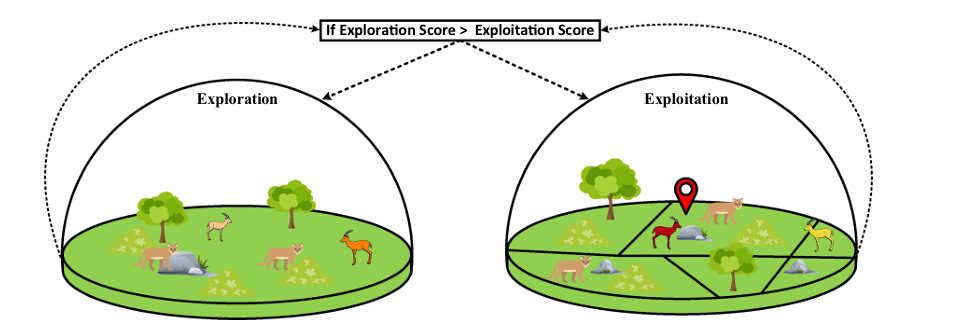
\includegraphics[width=0.9\textwidth]{Pictures/Screenshot 2025-10-27 235720.png}
\caption{Phase transition mechanism in the Puma Optimizer (POA).}
\label{fig:phase_transition}
\end{figure}


\subsubsection*{(d) Exploration Operation}
In the exploration stage, pumas roam randomly to identify promising areas within their territory. Candidate solutions are generated as
\begin{equation}
Z_{i,G} =
\begin{cases}
R_{pum} \times (U_b - L_b) + L_b, & \text{if } rand_1 > 0.5, \\
X_{a,G} + G \cdot ((X_{a,G} - X_{b,G}) + (X_{c,G} - X_{d,G})), & \text{otherwise,}
\end{cases}
\end{equation}
\begin{equation}
G = 2 \cdot rand_2 - 1,
\end{equation}
where $X_{a,G}, X_{b,G}, X_{c,G}, X_{d,G}$ are randomly selected agents, and $R_{pum}$ is a random roaming parameter.

\subsubsection*{(e) Exploitation Operation}
In the exploitation (ambush) phase, two sub-mechanisms—ambush and sprint—simulate pumas’ hunting strategies. The position update rule is expressed as
\begin{equation}
X_{new} =
\begin{cases}
\frac{\text{mean}(Sol_{total})}{N_{pop}} \cdot X_i - (-1)^{rand_3} \cdot X_i, & \text{if } rand_4 \geq 0.5,\\
Puma_{male} + (2 \cdot rand_5) \cdot exp(rand_6) \cdot (X^T_i - X_i), & \text{otherwise,}
\end{cases}
\end{equation}
where $Sol_{total}$ is the sum of all solutions, $Puma_{male}$ is the global best solution, $X^T_i$ is a randomly selected agent, and $rand_k$ are random values in $[0,1]$. Equations (34)--(38) in the original formulation define auxiliary coefficients:
\begin{equation}
R = 2 \cdot rand_{11} - 1, \quad
F_1 = rand_{12} \cdot exp\left(2 - Iter \cdot \frac{2}{MaxIter}\right), \quad
F_2 = w (v)^2 \cdot cos(2 \cdot rand_{13}) \cdot w.
\end{equation}

\subsubsection*{(f) Computational Complexity}
The computational complexity of POA can be summarized as
\begin{equation}
O\big((2T + 1)N^2 \times N \times D\big)
\end{equation}

where $N$ is the number of agents, $T$ is the maximum iteration count, and $D$ is the dimensionality of the search space. The initialization and fitness evaluation stages contribute $O(N)$ complexity, while the exploration and exploitation updates dominate overall runtime.

\begin{figure}[h!]
\centering
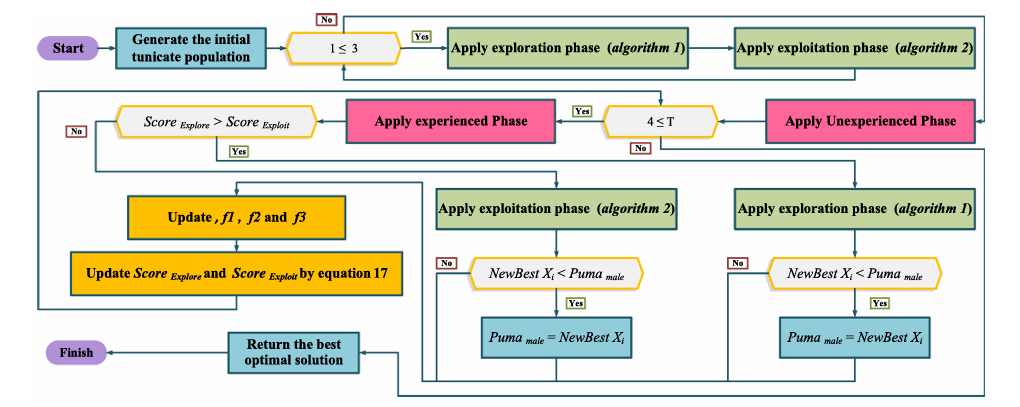
\includegraphics[width=0.9\textwidth]{Pictures/Screenshot 2025-10-28 000533.png}
\caption{POA Procedure}
\label{fig:POA_Procedure}
\end{figure}

\vspace{0.3cm}
In summary, the mathematical model captures the two-level adaptive intelligence of POA: a learning-driven unexperienced phase that builds search diversity and an experienced phase that dynamically alternates between exploration and exploitation based on performance scoring. This adaptive mechanism forms the baseline of the proposed hybrid HPO model, where the exploitation stage is further enhanced by PSO’s velocity--position learning.
\vspace{0.5em}
\noindent For a detailed mathematical derivation and extended explanation of each phase of the Puma Optimizer, readers are referred to the original paper: 
\textit{Puma optimizer (PO): a novel metaheuristic optimization algorithm}, available at 
\small{\href{https://www.mathworks.com/matlabcentral/fileexchange/157231-puma-optimizer-po}{\texttt{Puma Optimizer}}}.

\subsection{Mathematical Model of Particle Swarm Optimization (PSO)}

Particle Swarm Optimization (PSO) is a population-based stochastic optimization algorithm inspired by the collective social behavior of bird flocks and fish schools. In PSO, each particle represents a potential solution that moves through the search space according to its own experience and that of its neighbors. This cooperative learning process enables particles to exchange information dynamically, allowing the swarm to converge toward promising regions of the search space. PSO is particularly known for its fast convergence rate and strong local exploitation ability.

Let $X_i^t = [x_{i1}^t, x_{i2}^t, \ldots, x_{iD}^t]$ denote the position of the $i$-th particle at iteration $t$ in a $D$-dimensional search space, and let $V_i^t = [v_{i1}^t, v_{i2}^t, \ldots, v_{iD}^t]$ represent its velocity vector. The position of each particle is iteratively updated using the following equations:
\begin{equation}
V_i^{t+1} = w V_i^{t} + c_1 r_1 (Pbest_i - X_i^{t}) + c_2 r_2 (Gbest - X_i^{t}),
\end{equation}
\begin{equation}
X_i^{t+1} = X_i^{t} + V_i^{t+1},
\end{equation}
where:
\begin{itemize}
    \item $w$ is the inertia weight that controls the influence of the previous velocity on the current movement.
    \item $c_1$ and $c_2$ are acceleration coefficients representing cognitive (self-learning) and social (swarm-learning) components, respectively.
    \item $r_1$ and $r_2$ are uniformly distributed random numbers in the interval $[0,1]$.
    \item $Pbest_i$ is the personal best position found by the $i$-th particle up to iteration $t$.
    \item $Gbest$ is the global best position found by the entire swarm.
\end{itemize}

The first term in Eq.~(16) maintains the particle's momentum, the second term pulls it toward its own best-known position, and the third term attracts it toward the swarm's global best. The balance among these three components determines the trade-off between exploration and exploitation. To prevent excessive velocity leading to divergence, the velocity is often clamped as:
\begin{equation}
V_i^{t+1} = 
\begin{cases}
V_{max}, & \text{if } V_i^{t+1} > V_{max}, \\
-V_{max}, & \text{if } V_i^{t+1} < -V_{max}, \\
V_i^{t+1}, & \text{otherwise.}
\end{cases}
\end{equation}

The inertia weight $w$ decreases linearly during the search process to promote exploration at early stages and exploitation in later iterations:
\begin{equation}
w = w_{max} - \frac{t}{T} (w_{max} - w_{min}),
\end{equation}
where $t$ is the current iteration, and $T$ is the maximum number of iterations. This adaptive adjustment of $w$ is essential for maintaining convergence stability and avoiding local entrapment.

To further enhance convergence, an improved velocity normalization technique can be used:
\begin{equation}
V_i^{t+1} = \frac{V_i^{t+1}}{\|V_i^{t+1}\| + \epsilon},
\end{equation}
where $\epsilon$ is a small constant to avoid division by zero, ensuring numerical stability in high-dimensional problems.

At each iteration, the fitness function $f(X_i^{t})$ is evaluated for all particles. The individual and global bests are updated as:
\begin{equation}
Pbest_i =
\begin{cases}
X_i^{t}, & \text{if } f(X_i^{t}) < f(Pbest_i), \\
Pbest_i, & \text{otherwise,}
\end{cases}
\qquad
Gbest = \arg\min f(Pbest_i).
\end{equation}

The iterative process continues until the maximum iteration count $T$ is reached or convergence criteria are satisfied. The final global best $Gbest$ represents the optimal or near-optimal solution found by the swarm.

\subsubsection*{Computational Complexity}
For a swarm of $N_{pop}$ particles, a problem of dimension $D$, and $T$ iterations, the computational complexity of PSO can be expressed as:
\begin{equation}
O(N_{pop} \times D \times T),
\end{equation}
which is linear with respect to population size and dimensionality. This efficiency, combined with its simplicity and rapid convergence, makes PSO an ideal candidate for hybridization with other metaheuristic algorithms.
\begin{figure}[h!]
  \centering
  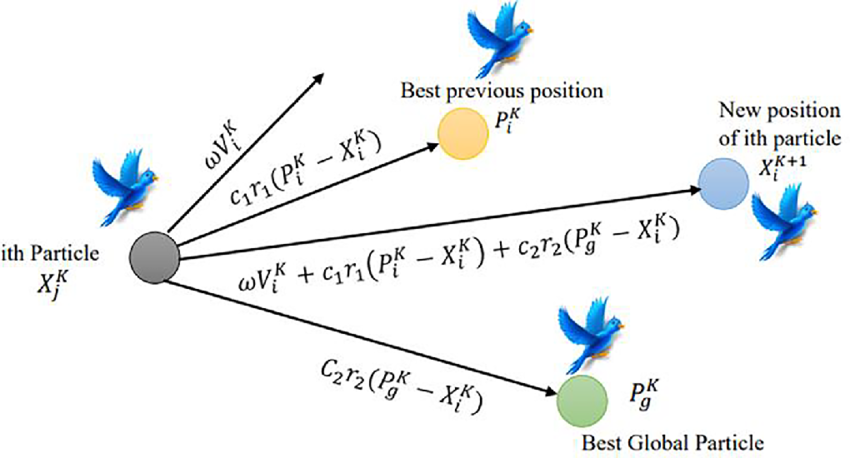
\includegraphics[width=0.9\textwidth]{Pictures/Particle-Swarm-Optimization-Architecture-Illustration.png}
  \caption{Schematic diagram of Particle Swarm Optimization (PSO).}
  \label{fig:pso_schema}
\end{figure}

\vspace{0.4em}
In the proposed Hybrid PUMA--PSO Optimizer (HPO), the velocity--position update rule of PSO is strategically embedded within the exploitation (ambush) phase of PUMA to accelerate convergence and improve local search efficiency. The details of this integration are described in Section~2.4.

\subsection{Hybridization Strategy of the Hybrid PUMA--PSO Optimizer (HPO)}

The proposed \textbf{Hybrid PUMA--PSO Optimizer (HPO)} introduces a cooperative hybridization strategy in which a short-run Particle Swarm Optimization (PSO) process refines elite solutions generated by the Puma Optimizer (POA). Unlike traditional blended hybrids that merge position-update rules, HPO employs a \textit{two-level embedded mechanism} where PSO acts as a local enhancement operator inside POA’s exploitation phase. This design retains POA’s strong global exploration ability while injecting PSO’s rapid convergence behavior only where it is most beneficial.

\subsubsection*{(a) Motivation for Hybridization}
Empirical studies of POA reveal that its exploitation stage tends to stagnate once the population diversity decreases, leading to slower convergence near the optimum. While POA excels at discovering promising regions through adaptive phase switching, its local refinement is limited by the absence of cooperative feedback among agents. To overcome this, PSO is integrated as a micro-level optimizer operating selectively on the best-performing agents, accelerating convergence without disrupting the overall population dynamics.

\subsubsection*{(b) Integration Mechanism}
The hybridization takes place after the completion of POA’s standard exploitation phase in each iteration. The integration steps are as follows:
\begin{enumerate}
    \item Run POA’s standard exploration and exploitation phases for one iteration.
    \item Rank all solutions by fitness and select the top $k_{refine}$ elite agents:
    \[
    Elite = \{X_{(1)}, X_{(2)}, \ldots, X_{(k_{refine})}\}, \quad f(X_{(1)}) \le f(X_{(2)}) \le \cdots
    \]
    \item Initialize a micro-PSO subsystem using these elite agents as the initial population. The PSO update equations are:
    \[
    V_i^{t+1} = \omega V_i^t + c_1 r_1 (Pbest_i - X_i^t) + c_2 r_2 (Gbest - X_i^t),
    \]
    \[
    X_i^{t+1} = X_i^t + V_i^{t+1}.
    \]
    \item Execute the micro-PSO for $T_{micro}$ iterations (typically $5$--$10$) to locally refine the elite positions.
    \item Replace the original elite agents in the POA population with their refined versions:
    \[
    X_{(i)}^{new} = X_{(i)}^{refined}, \quad i = 1,2,\ldots,k_{refine}.
    \]
\end{enumerate}
This cooperative mechanism allows the global population to continue evolving under POA’s adaptive strategy, while elite members undergo targeted fine-tuning through PSO’s memory-based learning.

\subsubsection*{(c) Control Parameters and Adaptation}
The number of elite agents $k_{refine}$ and the micro-PSO iteration count $T_{micro}$ are key parameters that determine computational cost and improvement depth. In practice, $k_{refine}$ is set as a small fraction (e.g., $5$--$10\%$) of the total population, while $T_{micro}$ is limited to avoid excessive overhead. To ensure adaptive refinement, $k_{refine}$ can increase slightly with iterations according to:
\begin{equation}
k_{refine}(t) = \left\lceil k_{min} + \frac{t}{T}(k_{max} - k_{min}) \right\rceil,
\end{equation}
where $T$ is the maximum iteration count. This enables stronger exploitation in later stages.

% \subsubsection*{(d) Algorithmic Flow of HPO}
% Figure~\ref{fig:hpo_framework} (to be added later) will illustrate the overall workflow. The summarized procedure is:
% \begin{itemize}
%     \item Initialize POA population and parameters.
%     \item Execute adaptive phase switching (unexperienced/experienced) as in POA.
%     \item Perform standard POA updates (exploration and exploitation).
%     \item Select elite agents and refine them using micro-PSO for $T_{micro}$ iterations.
%     \item Replace refined elites and continue to the next iteration.
% \end{itemize}
% This approach enables HPO to maintain high diversity in early iterations while applying PSO-driven local optimization later in the process.

\subsubsection*{(e) Discussion on Hybrid Effectiveness}
By limiting PSO operations to a small elite subset, HPO achieves the benefits of fast convergence without sacrificing scalability. The cooperation between POA’s adaptive intelligence and PSO’s collective learning enhances both search precision and convergence rate. The hybridization is lightweight yet powerful—requiring only minor additional computation but significantly improving exploitation performance.

\vspace{0.5em}
A step-by-step algorithm and pseudocode representation of the complete HPO algorithm is presented in Section~2.5.

\subsection{Algorithmic Steps and Pseudocode of the Hybrid PUMA--PSO Optimizer (HPO)}

The proposed \textbf{Hybrid PUMA--PSO Optimizer (HPO)} operates through a sequence of adaptive exploration, exploitation, and elite refinement processes. The following steps summarize the complete workflow of the algorithm, corresponding to the flowchart shown in Fig.~\ref{fig:hpo_flowchart}.

\begin{enumerate}
    \item \textbf{Initialization:} 
    \begin{itemize}
        \item Define the objective function $f(\mathbf{x})$ to be minimized (or maximized).
        \item Set algorithmic parameters: population size $N_{pop}$, search-space bounds $(L_b, U_b)$, phase coefficients $(PF_1, PF_2, PF_3)$, number of elites $k_{refine}$, micro-PSO iteration count $T_{micro}$, and maximum iteration count $T$.
        \item Initialize the positions of all pumas $X_i$ randomly within the bounds and evaluate their fitness.
    \end{itemize}

    \item \textbf{Phase Classification:}
    \begin{itemize}
        \item Determine whether the current iteration belongs to the \textit{unexperienced} or \textit{experienced} phase according to iteration ratio or adaptive score metrics.
        \item In the unexperienced phase, allow both exploration and exploitation updates to run sequentially to establish base performance knowledge.
        \item In the experienced phase, choose between exploration or exploitation based on the comparative scores $Score_{Explor}$ and $Score_{Exploit}$.
    \end{itemize}

    \item \textbf{Standard POA Update:}
    \begin{itemize}
        \item Execute the corresponding POA operation (exploration, stalking, or ambush) using the mathematical model described in Section~2.2.
        \item Evaluate the fitness of the updated agents and update the current best solution $X^*$.
    \end{itemize}

    \item \textbf{Elite Selection:}
    \begin{itemize}
        \item Sort all solutions by fitness value.
        \item Select the top $k_{refine}$ elite agents:
        \[
        Elite = \{ X_{(1)}, X_{(2)}, \ldots, X_{(k_{refine})} \}.
        \]
    \end{itemize}

    \item \textbf{Micro-PSO Refinement:}
    \begin{itemize}
        \item Initialize a small PSO subsystem using the elite agents as particles; assign random or zero initial velocities.
        \item For $T_{micro}$ iterations:
        \begin{enumerate}
            \item Update velocities and positions using PSO equations:
            \[
            V_i^{t+1} = \omega V_i^t + c_1 r_1 (Pbest_i - X_i^t) + c_2 r_2 (Gbest - X_i^t),
            \]
            \[
            X_i^{t+1} = X_i^t + V_i^{t+1}.
            \]
            \item Evaluate fitness, update personal and global bests within the micro-PSO group.
        \end{enumerate}
        \item Replace the original elite solutions in the POA population with their refined versions.
    \end{itemize}

    \item \textbf{Population Update:}
    \begin{itemize}
        \item Re-evaluate the entire population’s fitness after refinement.
        \item Update the global best $Gbest$ and increment the iteration counter.
    \end{itemize}

    \item \textbf{Termination Check:}
    \begin{itemize}
        \item If the maximum number of iterations $T$ is reached or the improvement in $Gbest$ falls below a predefined threshold, stop the search.
        \item Otherwise, return to Step 2 and continue the adaptive loop.
    \end{itemize}

    \item \textbf{Output:}
    \begin{itemize}
        \item Return the final best solution $Gbest$ and its objective value $f(Gbest)$ as the optimal result.
    \end{itemize}
\end{enumerate}

\vspace{0.4em}
The above procedure encapsulates the cooperation between POA’s adaptive phase transitions and PSO’s memory-driven local refinement. This synergy ensures that global exploration is maintained while convergence toward the global optimum is significantly accelerated.

\begin{figure}[h!]
  \centering
  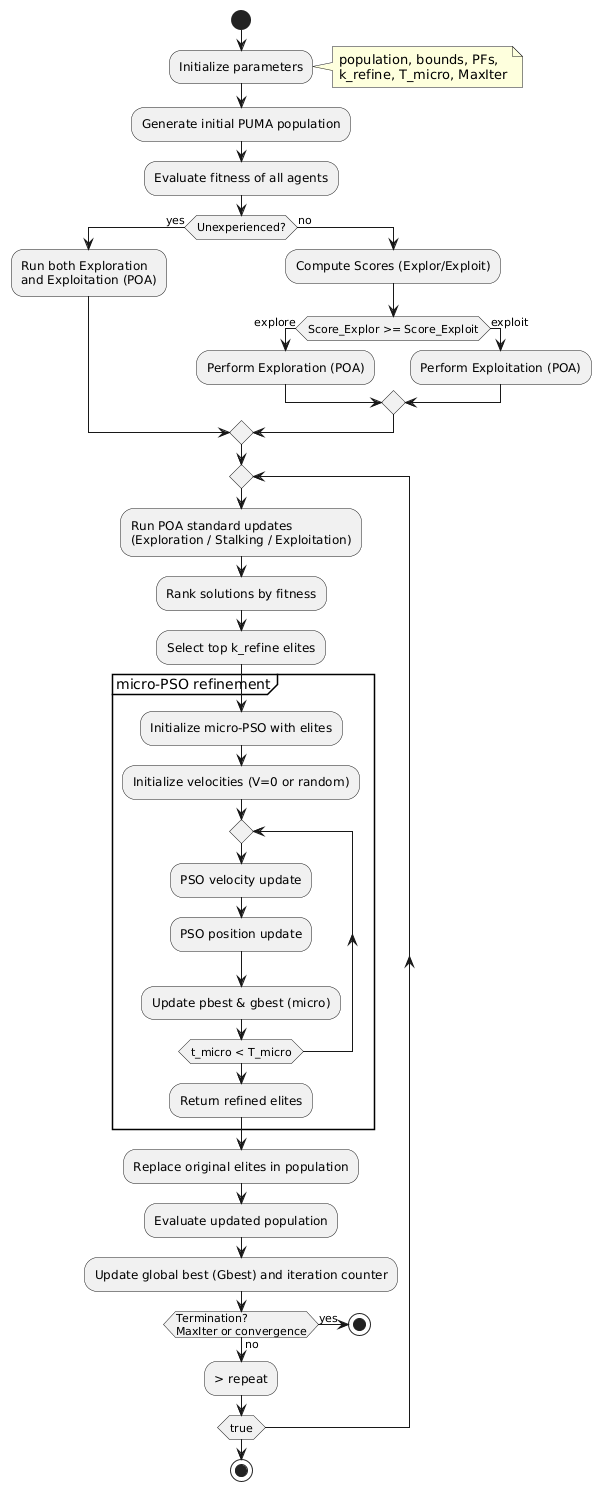
\includegraphics[width=0.5\textwidth]{Pictures/hpo.png}
  \caption{HPO Flowchart}
  \label{fig:hpo_flowchart}
\end{figure}

Similarly the psuedocode for HPO can be given as
% Put these in the preamble if not already present:

\begin{algorithm}
\footnotesize
\caption{Pseudo-code of the Hybrid PUMA--PSO Optimizer (HPO)}
\label{alg:hpo}
\begin{algorithmic}[1]
\Require $f(\cdot)$ objective function, population size $N_{pop}$, problem bounds $L_b,U_b$, max iterations $T$,\\
\quad POA parameters $(PF_1,PF_2,PF_3, \ldots)$, micro-PSO params $(k_{refine}, T_{micro}, \omega, c_1, c_2, V_{max})$
\Ensure Best solution $Gbest$ and $f(Gbest)$
\vspace{0.5em}

\State \textbf{Initialization:}
\For{$i \leftarrow 1$ to $N_{pop}$}
    \State $X_i \leftarrow L_b + \mathrm{rand}(0,1)\cdot (U_b-L_b)$ \Comment{random initial positions}
    \State $f_i \leftarrow f(X_i)$
    \State $Pbest_i \leftarrow X_i$
\EndFor
\State $Gbest \leftarrow \arg\min_i f_i$
\State set iteration $t \leftarrow 1$
\State initialize any POA internal sequences / counters (SeqCosts, SeqTimes, etc.)

\vspace{0.4em}
\While{$t \le T$}
    \Comment{Phase decision: Unexperienced (initial reps) or Experienced}
    \If{t $\le$ $t_{unexp}$} \Comment{Unexperienced: run both phases to build baseline}
        \State Apply POA Exploration Phase (see Algorithm~\ref{alg:po_explore})
        \State Apply POA Exploitation Phase (see Algorithm~\ref{alg:po_exploit})
    \Else
        \State Compute $Score_{Explor}$ and $Score_{Exploit}$ (POA scoring functions)
        \If{$Score_{Explor} \ge Score_{Exploit}$}
            \State Apply POA Exploration Phase
        \Else
            \State Apply POA Exploitation Phase
        \EndIf
    \EndIf

    \State Evaluate all solutions $\{X_i\}$ and update $f_i$
    \State Update $Pbest_i$ for all particles and $Gbest \leftarrow \arg\min_i Pbest_i$

    \vspace{0.3em}
    \State \textbf{Elite selection:}
    \State Sort solutions by fitness ascending and select elites
    \State $Elite \leftarrow \{X_{(1)}, X_{(2)}, \dots, X_{(k_{refine})}\}$

    \vspace{0.3em}
    \State \textbf{Micro-PSO refinement:}
    \Comment{Initialize micro-PSO population with the elites}
    \For{each elite $j=1\ldots k_{refine}$}
        \State $x_j^{(0)} \leftarrow X_{(j)}$
        \State $v_j^{(0)} \leftarrow \text{rand or }0$
        \State $pbest_j \leftarrow x_j^{(0)}$
    \EndFor
    \State $g_{micro} \leftarrow \arg\min_j f(pbest_j)$
    \For{$\tau \leftarrow 1$ to $T_{micro}$}
        \For{each micro-particle $j=1\ldots k_{refine}$}
            \State $v_j \leftarrow \omega v_j + c_1 r_1 (pbest_j - x_j) + c_2 r_2 (g_{micro} - x_j)$
            \State clamp $v_j$ to $[-V_{max},V_{max}]$
            \State $x_j \leftarrow x_j + v_j$
            \State enforce bounds: $x_j \in [L_b,U_b]$
            \State $f_j \leftarrow f(x_j)$
            \If{$f_j < f(pbest_j)$}
                \State $pbest_j \leftarrow x_j$
            \EndIf
        \EndFor
        \State $g_{micro} \leftarrow \arg\min_j f(pbest_j)$
    \EndFor

    \vspace{0.3em}
    \State \textbf{Replace elites:}
    \For{$j \leftarrow 1$ to $k_{refine}$}
        \State Replace $X_{(j)} \leftarrow pbest_j$ (or $x_j$ depending on policy)
        \State Update corresponding $f_{(j)} \leftarrow f(pbest_j)$
    \EndFor

    \vspace{0.3em}
    \State Update global memory: update $Pbest_i$ and $Gbest$ if improved
    \State Update POA sequences / costs / scores for next iteration
    \State $t \leftarrow t + 1$
\EndWhile

\State \Return $Gbest, f(Gbest)$
\end{algorithmic}
\end{algorithm}

\begin{algorithm}[h!]
\footnotesize
\caption{Pseudo-code of the Exploration Phase of PUMA}
\label{alg:po_explore}
\begin{algorithmic}[1]
\State \textbf{Input:} Population $\{X_i\}_{i=1}^{N_{pop}}$, bounds $(L_b,U_b)$
\State \textbf{Output:} Updated population after exploration
\vspace{0.2em}
\State Sort population in ascending order by cost
\State Calculate the parameter $p$ using Eq.~(29)
\For{each puma $X_i$}
    \State Randomly select four solutions $X_a,X_b,X_c,X_d$
    \State Compute a new vector $Z_i$ using Eq.~(25)--(26)
    \State Check the boundary of $Z_i$; if outside, clip to $[L_b,U_b]$
    \State Evaluate cost $f(Z_i)$
    \If{$f(Z_i) < f(X_i)$}
        \State $X_i \leftarrow Z_i$ \Comment{Accept improved solution}
    \Else
        \State $U \leftarrow U + p$ \Comment{Update the control parameter}
    \EndIf
\EndFor
\State \Return Updated population $\{X_i\}$
\end{algorithmic}
\end{algorithm}

\begin{algorithm}[h!]
\footnotesize
\caption{Pseudo-code of the Exploitation Phase of PUMA}
\label{alg:po_exploit}
\begin{algorithmic}[1]
\State \textbf{Input:} Current population $\{X_i\}$, global best $Puma_{male}$
\State \textbf{Output:} Updated population after exploitation
\vspace{0.2em}
\For{each puma $X_i$}
    \State Calculate parameters $R$, $F_1$, and $F_2$ using Eqs.~(34)--(36)
    \State Generate new candidate solution $NewX_i$ using Eq.~(32)
    \State Evaluate $f(NewX_i)$
    \If{$f(NewX_i) < f(X_i)$}
        \State $X_i \leftarrow NewX_i$
    \EndIf
\EndFor
\State \Return Updated population $\{X_i\}$
\end{algorithmic}
\end{algorithm}

\subsection{Computational Complexity Analysis}

The computational complexity of the proposed \textbf{Hybrid PUMA--PSO Optimizer (HPO)} depends on the number of search agents, problem dimensionality, and the number of iterations. Each iteration of the algorithm involves three major computational stages: (i) the standard PUMA operations (exploration and exploitation), (ii) the micro-PSO refinement of elite solutions, and (iii) fitness evaluations.

Let $N_{pop}$ denote the population size, $D$ the dimensionality of the problem, and $T$ the maximum number of iterations. The computational cost for the main PUMA procedure can be expressed as:
\begin{equation}
O_{POA} = O\big(N^2 D T\big).
\end{equation}
since each iteration updates $N_{pop}$ solutions of $D$ dimensions and evaluates their objective function values.

The hybrid micro-PSO refinement is executed on only a small subset of the population, namely the top $k_{refine}$ elite agents, for $T_{micro}$ inner iterations. The additional cost introduced by this process is:
\begin{equation}
O_{micro} = O\big(k_{\mathrm{refine}} \, D \, T_{\mathrm{micro}}\big).
\end{equation}
Because $k_{refine} \ll N_{pop}$ and $T_{micro} \ll T$, the micro-PSO step contributes only a small constant overhead to the overall runtime. Therefore, the total computational complexity of HPO can be approximated as:
\begin{equation}
O_{HPO} = O\big(N^2 D T\big) + O\big(k_{\mathrm{refine}} \, D \, T_{\mathrm{micro}}\big)
\approx O\big(N^2 D T\big),
\end{equation}

The asymptotic complexity remains linear with respect to both population size and problem dimensionality, similar to the base PUMA and PSO algorithms. However, the micro-PSO refinement introduces a negligible constant factor that slightly increases runtime while significantly improving convergence accuracy and solution stability. Empirical results (Section~3) demonstrate that the hybrid achieves better performance without substantial computational overhead.

\section{Experimental Results and Discussion}
\subsection{Experimental Setup}

To evaluate the proposed Hybrid PUMA--PSO Optimizer (HPO), all experiments were conducted in an open-source MATLAB-compatible environment using \textbf{GNU Octave 8.3.0}. 
The computational setup consisted of an \textbf{AMD Ryzen 7 7840HS} processor (3.8~GHz base frequency, 8 cores, 16 threads), \textbf{16~GB RAM}, and the \textbf{Windows~11} operating system.

The implementation was based on the official PUMA Optimizer (PO) source code provided by Abdollahzadeh \textit{et~al.}~\cite{puma2023}, which was modified to incorporate additional instrumentation for exploitation tracking and a PSO-based hybridization module. 
All algorithms were implemented in \texttt{.m} scripts compatible with MATLAB syntax.

\subsubsection{Algorithm Parameters}
For a fair comparison, both the original PUMA and the proposed Hybrid PUMA--PSO were executed under identical experimental settings. 
Table~\ref{tab:params} summarizes the general parameter configuration used throughout all tests.

\begin{table}[h!]
\centering
\caption{General Parameter Settings for PUMA and Hybrid PUMA--PSO}
\label{tab:params}
\begin{tabular}{@{}llcl@{}}
\toprule
\textbf{Parameter} & \textbf{Symbol} & \textbf{Value} & \textbf{Description} \\ \midrule
Population size & $n_{sol}$ & 30 & Number of search agents \\
Maximum iterations & $T$ & 500 & Termination criterion \\
Dimensionality & $D$ & 30 & Number of decision variables \\
Search range & $[lb, ub]$ & Function-specific & Lower and upper bounds \\
Independent runs & $R$ & 30 & Statistical evaluation \\ \bottomrule
\end{tabular}
\end{table}

\subsubsection{Hybridization Parameters}
The proposed HPO retains the original PUMA exploration and exploitation stages. 
After each exploitation phase, a micro-PSO is applied to the top-performing solutions (elite set) to enhance local refinement and accelerate convergence toward the optimum. 
The configuration for this PSO-based refinement is presented in Table~\ref{tab:hybridparams}.

\begin{table}[h!]
\centering
\caption{Micro-PSO Refinement Parameters}
\label{tab:hybridparams}
\begin{tabular}{@{}llcl@{}}
\toprule
\textbf{Parameter} & \textbf{Symbol} & \textbf{Value} & \textbf{Description} \\ \midrule
Elite count & $k_{e}$ & 5 & Number of elite solutions refined by PSO \\
Micro-PSO iterations & $L$ & 8 & Local PSO refinement steps \\
Inertia weight & $w$ & 0.7 & Balances exploration and exploitation in PSO \\
Cognitive coefficient & $c_{1}$ & 1.5 & Self-learning factor \\
Social coefficient & $c_{2}$ & 1.5 & Collective-learning factor \\
Max velocity scaling & $v_{\max}$ & $0.1\times(ub-lb)$ & Controls particle step size \\ \bottomrule
\end{tabular}
\end{table}

\subsubsection{Performance Evaluation Setup}
Both algorithms were tested on seven standard \textbf{unimodal benchmark functions (F1--F7)} to evaluate convergence behavior, exploitation strength, and accuracy. 
Each algorithm was executed for 30 independent runs on every function to ensure statistical validity.

The following performance metrics were recorded:
\begin{itemize}
    \item Mean, median, and standard deviation of the final best cost values.
    \item Mean late-exploitation rate and convergence slope (indicators of exploitation activity).
    \item Fraction of runs showing improvement in the final 20\% of iterations.
\end{itemize}

The significance of performance differences was validated using the \textbf{Wilcoxon rank-sum test} and \textbf{Cohen’s~d} effect size analysis. 
All convergence histories, exploitation activity logs, and statistical summaries were stored automatically in \texttt{.mat} and \texttt{.csv} formats for subsequent analysis.

\bigskip
The proposed experimental setup ensures that the hybridization results are reproducible, statistically sound, and directly comparable with the baseline PUMA algorithm.

\subsection{Benchmark Functions (F1--F7)}

To evaluate the optimization performance and exploitation capability of both algorithms, seven standard \textbf{unimodal benchmark functions} ($F_1$--$F_7$) were used.  
These functions are widely adopted in metaheuristic research because they offer known global minima and analytical expressions, enabling a precise evaluation of convergence behavior and exploitation strength.  
Unimodal functions have only one global optimum, making them ideal for testing an algorithm’s local search efficiency and precision.

\subsubsection{Mathematical Definitions}

The benchmark functions used in this study are defined as follows:

\begin{equation}
F_1(x) = \sum_{i=1}^{D} x_i^2
\end{equation}
A simple convex function with a bowl-shaped surface. Tests convergence speed and precision.

\begin{equation}
F_2(x) = \sum_{i=1}^{D} |x_i| + \prod_{i=1}^{D} |x_i|
\end{equation}
Combines additive and multiplicative terms, evaluating an algorithm's balance between search directions.

\begin{equation}
F_3(x) = \sum_{i=1}^{D} \left( \sum_{j=1}^{i} x_j \right)^2
\end{equation}
The Schwefel 1.2 function introduces cumulative error propagation, testing stability and accuracy.

\begin{equation}
F_4(x) = \max_{i} \left( |x_i| \right)
\end{equation}
The Schwefel 2.21 function emphasizes worst-dimension performance and robustness of the optimizer.

\begin{equation}
F_5(x) = \sum_{i=1}^{D-1} \left[ 100(x_{i+1} - x_i^2)^2 + (x_i - 1)^2 \right]
\end{equation}
The Rosenbrock function features a narrow curved valley leading to the global minimum.  
It is challenging for exploitation, as solutions must make fine, correlated adjustments to converge.

\begin{equation}
F_6(x) = \sum_{i=1}^{D} \left( \lfloor x_i + 0.5 \rfloor \right)^2
\end{equation}
A discontinuous step function with plateaus and ridges that test precision and local refinement.

\begin{equation}
F_7(x) = \sum_{i=1}^{D} i\,x_i^4 + \text{rand}[0,1)
\end{equation}
A quartic function with added uniform noise to simulate stochastic objective surfaces.  
It evaluates robustness and stability under random perturbations.

\bigskip

\subsubsection{Benchmark Function Summary}

Table~\ref{tab:benchmark} summarizes the key properties of all benchmark functions.  
The global minimum of each function is located at $\mathbf{x}^* = 0$, with an optimal value $f(\mathbf{x}^*) = 0$, except for the Rosenbrock function ($F_5$), whose minimum lies at $\mathbf{x}^* = [1,1,\dots,1]$.

\begin{table}[h!]
\centering
\caption{Summary of Benchmark Functions (F1--F7)}
\label{tab:benchmark}
\begin{tabular}{@{}lllll@{}}
\toprule
\textbf{Func.} & \textbf{Name} & \textbf{Equation Type} & \textbf{Search Range} & \textbf{Optimum Value} \\ \midrule
$F_1$ & Sphere & Convex, smooth & $[-100, 100]$ & 0 \\
$F_2$ & Schwefel 2.22 & Additive + multiplicative & $[-10, 10]$ & 0 \\
$F_3$ & Schwefel 1.2 & Cumulative quadratic & $[-100, 100]$ & 0 \\
$F_4$ & Schwefel 2.21 & Max-absolute term & $[-100, 100]$ & 0 \\
$F_5$ & Rosenbrock & Narrow curved valley & $[-30, 30]$ & 0 \\
$F_6$ & Step & Discontinuous & $[-100, 100]$ & 0 \\
$F_7$ & Quartic + Noise & Stochastic, quartic & $[-1.28, 1.28]$ & $\approx 0$ \\ \bottomrule
\end{tabular}
\end{table}

\bigskip

The \textbf{first four functions ($F_1$--$F_4$) are relatively simple convex landscapes} used to verify convergence and stability.  
The remaining \textbf{functions ($F_5$--$F_7$) are more complex, requiring precise local search to reach the optimum}.  
Hence, these benchmarks are particularly effective for demonstrating the improved \textbf{exploitation ability} of the Hybrid PUMA--PSO Optimizer compared to the original PUMA.

\subsection{Analysis of PUMA’s Exploitation Limitation}

This section investigates the exploitation behavior of the original PUMA Optimizer to identify the primary limitation that motivated the hybridization approach.  
Since unimodal benchmark functions possess a single global optimum, they are ideal for assessing an algorithm’s exploitation capability rather than its exploration potential.  
Hence, the functions $F_1$--$F_7$ were employed to analyze how effectively PUMA performs local refinement after reaching promising regions in the search space.

\subsubsection{Methodology}
To measure the extent of exploitation activity, a logging mechanism was integrated into the \texttt{Exploitation.m} file of the original PUMA implementation.  
This mechanism recorded every iteration in which a new best solution was found, forming the matrix $\texttt{PO\_EXPLOIT\_HISTORY}(r,i)$, where $r$ represents the run index and $i$ denotes the iteration number.  
From these logs, the following metrics were computed:

\begin{equation}
E_{\text{late}} = \frac{1}{R}\sum_{r=1}^{R} 
\frac{1}{T/2}\sum_{i=T/2}^{T}\text{success}_{r,i}
\end{equation}

where $\text{success}_{r,i}=1$ if iteration $i$ yielded an improvement, and $0$ otherwise.  
This \textit{mean late-exploitation rate} quantifies how frequently the algorithm continues to improve after half of its total iterations.

\subsubsection{Empirical Observations}
Fig.~\ref{fig:conv_f5} illustrates the median convergence curve for the Rosenbrock function ($F_5$).  
The best-so-far cost shows a steep decline during the initial 20--30 iterations, followed by an almost flat region extending for the remaining 470 iterations.  
This early convergence plateau indicates that PUMA’s local search activity diminishes significantly after reaching near-optimal zones.

\begin{figure}[h!]
    \centering
    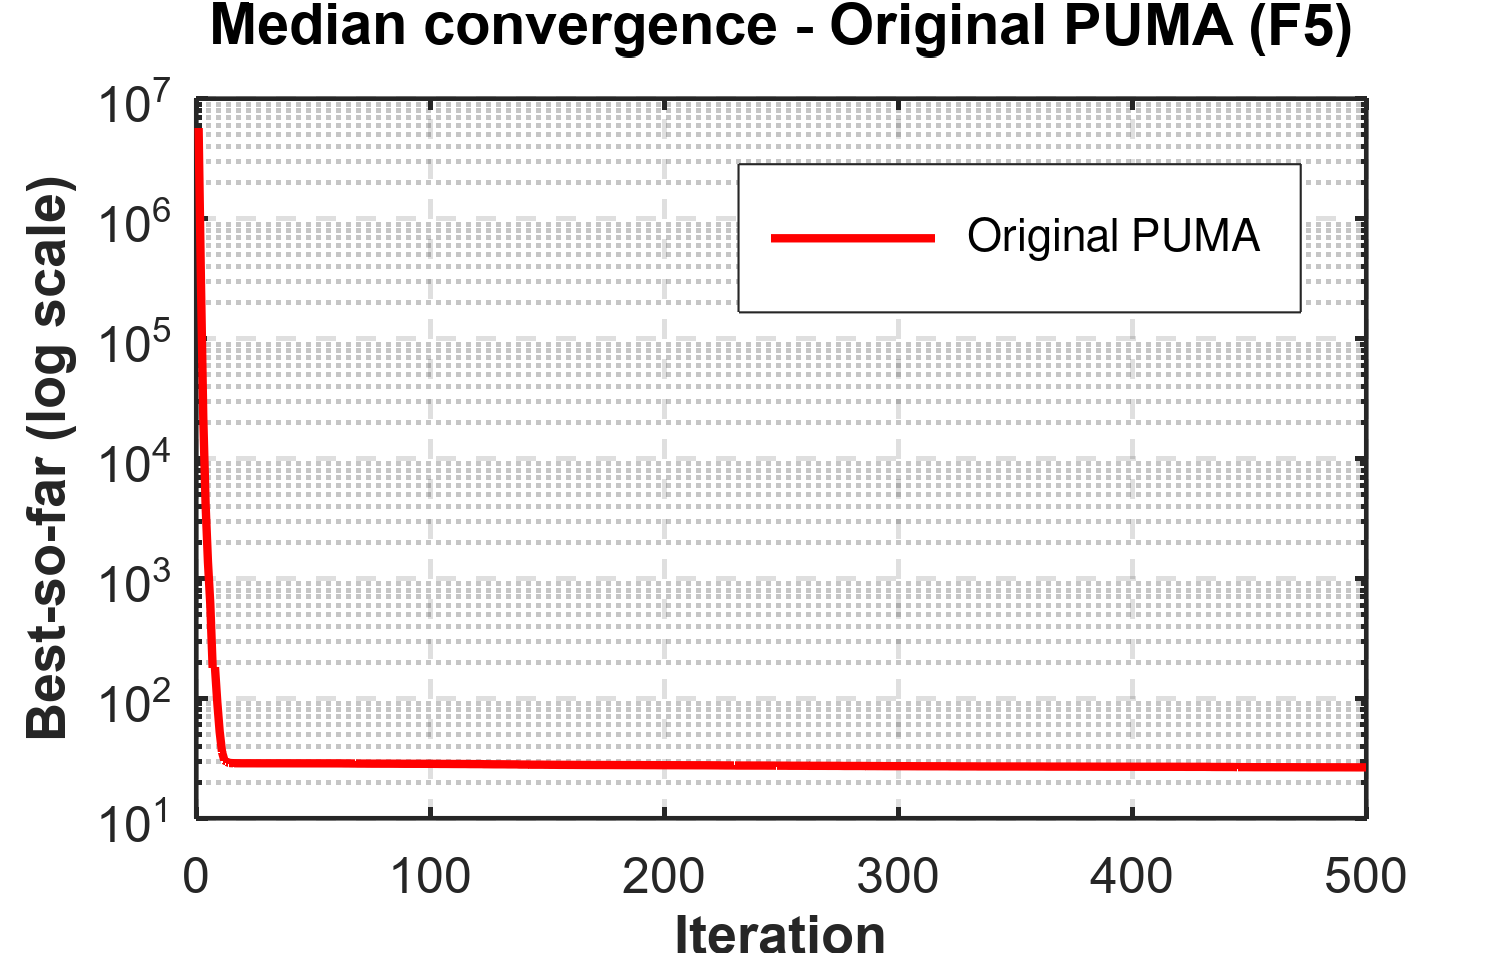
\includegraphics[width=0.70\linewidth]{Pictures/F5_PO_convergence_publication.png}
    \caption{Convergence curve of the original PUMA on $F_5$ (Rosenbrock function).  
    A sharp drop occurs during early iterations, followed by stagnation, indicating weak late-stage exploitation.}
    \label{fig:conv_f5}
\end{figure}


To further examine this behavior, the exploitation activity per iteration was visualized in Fig.~\ref{fig:po_exploit_multi}.  
The average number of successful exploitation events rapidly decreases and approaches zero after approximately 20--30 iterations for functions $F_5$, $F_6$, and $F_7$.  
This confirms that once PUMA locates a near-optimal region, it performs very few local refinements.

\subsubsection{Quantitative Analysis}
The quantitative summary extracted from 30 independent runs supports the above visual evidence.  
For instance, the mean late-exploitation rate $(E_{\text{late}})$ for $F_5$ and $F_6$ was recorded as approximately 0.77 and 0.70, respectively, compared to over 20 for simple convex functions ($F_1$--$F_4$).  
Furthermore, the median late-convergence slope approached zero ($\approx -10^{-4}$), signifying a lack of meaningful improvement in later iterations.

\begin{figure*}[t]
  \centering
  \subfloat[F5]{%
    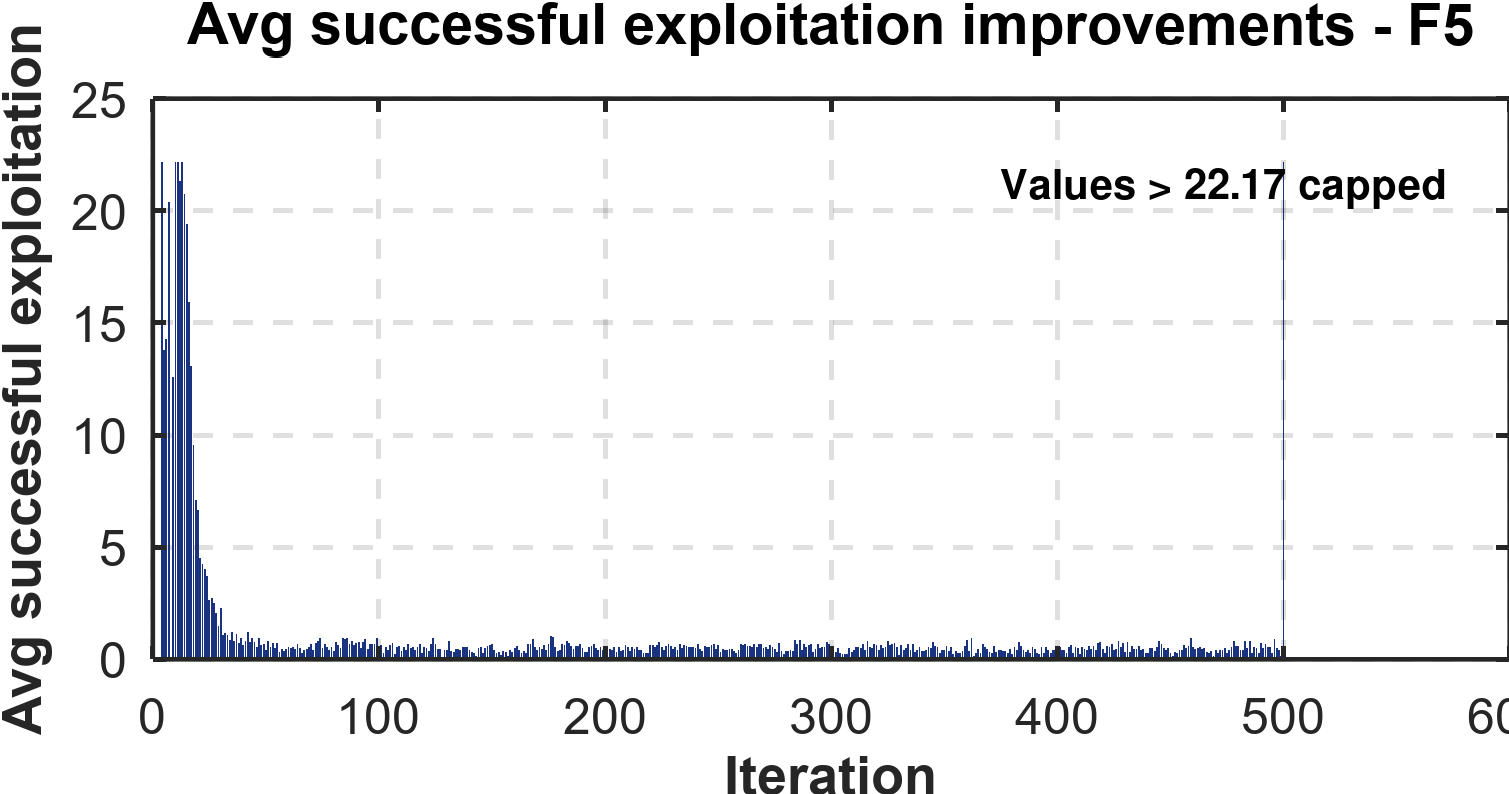
\includegraphics[width=0.32\textwidth]{Pictures/F5_exploit_activity_publication.png}
  }\hfill
  \subfloat[F6]{%
    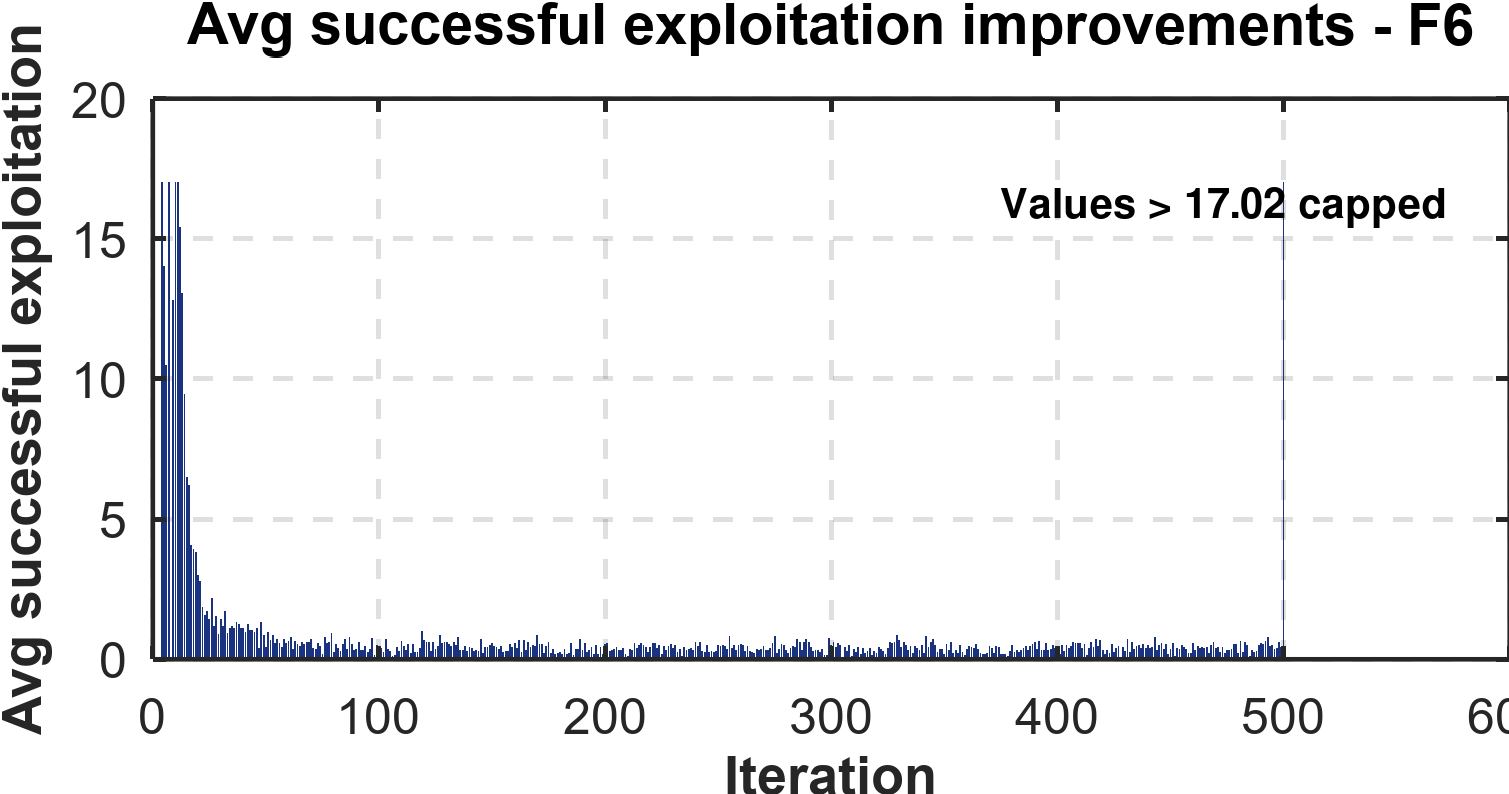
\includegraphics[width=0.32\textwidth]{Pictures/F6_exploit_activity_publication.png}
  }\hfill
  \subfloat[F7]{%
    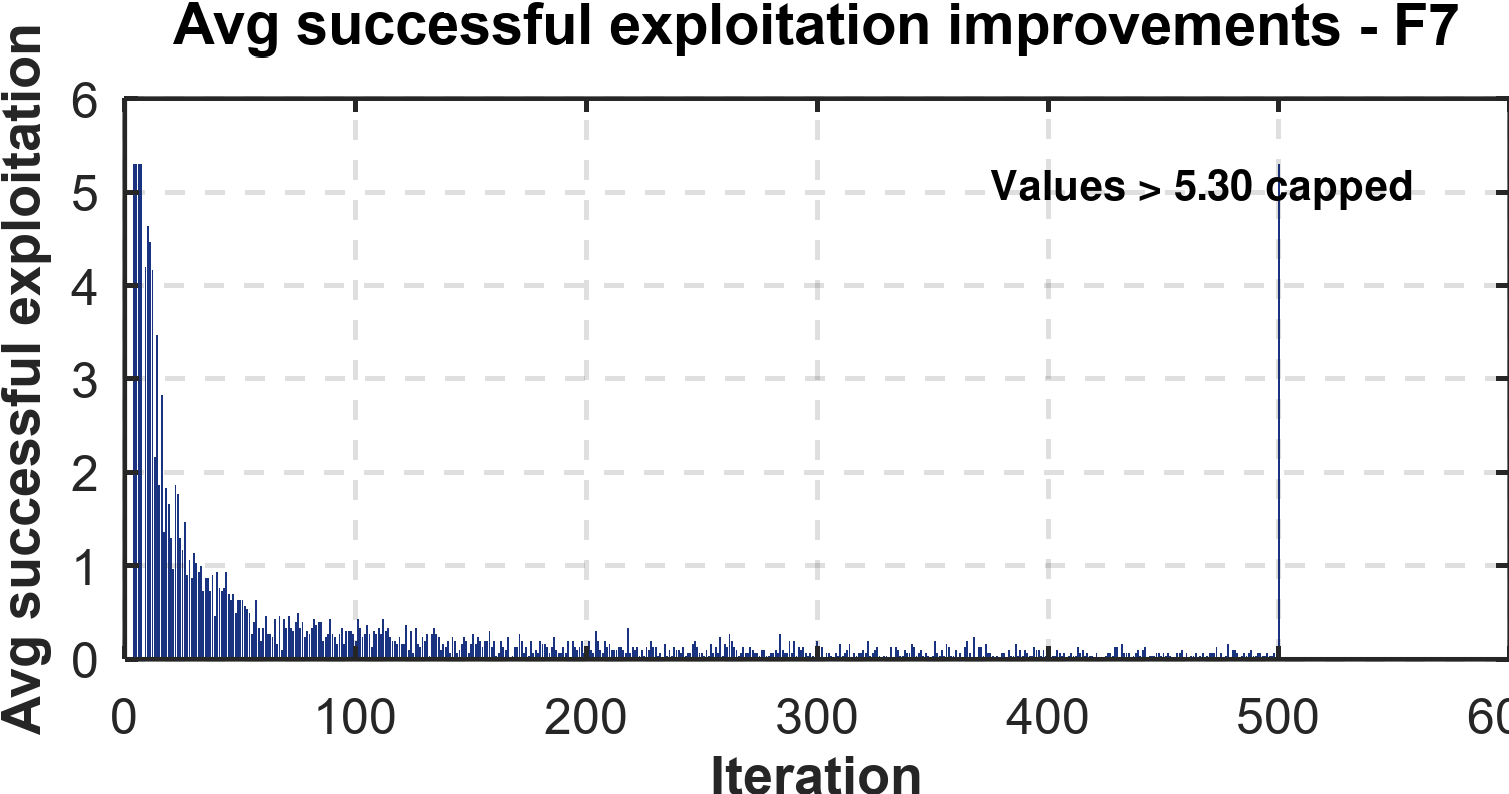
\includegraphics[width=0.32\textwidth]{Pictures/F7_exploit_activity_publication.png}
  }
  \caption{Average successful exploitation improvements per iteration for Original PUMA across benchmark functions $F_5$, $F_6$, and $F_7$. The rapid decline after the first 20--30 iterations demonstrates poor late-stage exploitation.}
  \label{fig:po_exploit_multi}
\end{figure*}

\subsubsection{Discussion}
The combined visual and quantitative analyses reveal that while PUMA exhibits strong exploration and rapid early convergence, its exploitation capability weakens considerably once it nears the global optimum.  
The algorithm fails to refine solutions within the narrow basins of attraction of functions such as Rosenbrock and Step.  
This stagnation behavior confirms that PUMA’s internal exploitation mechanism lacks sufficient local search pressure, thus motivating the introduction of a PSO-based refinement layer in the proposed Hybrid PUMA--PSO algorithm.

\subsection{Performance of Hybrid PUMA--PSO (HPO) vs PUMA}
\FloatBarrier 
\label{sec:performance_hpo_vs_po}

This section presents the quantitative comparison between the original Puma optimizer (PO) and the proposed hybrid (PUMA--PSO, denoted HPO). We evaluate both algorithms on the unimodal benchmark set ($F_1$--$F_7$). For each benchmark we report summary statistics (median, mean and standard deviation of final best fitness across 30 independent runs), and statistical test results comparing the distributions of final fitness values across the two algorithms.

\subsubsection{Quantitative metrics}
\label{sec:quant_metrics}

Table~\ref{tab:quant_metrics} summarizes the numerical comparison between PO and HPO. For each function we report the median and mean final best fitness observed across the 30 independent runs, the sample standard deviations, the two-sided Wilcoxon rank-sum test \(p\)-value, and Cohen's \(d\) effect size where computable. The Wilcoxon test is used because it is non-parametric and robust to non-Gaussian outcome distributions; we consider \(p<0.05\) as evidence that the difference is statistically significant. Cohen's \(d\) is reported as a standardized measure of effect magnitude (positive values indicate HPO performs better if medians / means are lower).

\begin{table*}[t]
\centering
\caption{Quantitative comparison of Original PUMA (PO) and Hybrid PUMA--PSO (HPO) on functions \(F_1\)–\(F_7\). Numbers report median, mean and standard deviation of the final best fitness (30 runs). `Wilcoxon\_p` is the two-sided Wilcoxon rank-sum \(p\)-value. `Cohen's d` is the effect size; `NaN` indicates an undefined value (see text).}
\label{tab:quant_metrics}
\resizebox{\textwidth}{!}{%
\begin{tabular}{lrrrrrrrc}
\toprule
Function & Median\_PO & Median\_HPO & Mean\_PO & Mean\_HPO & Std\_PO & Std\_HPO & Wilcoxon\_p & Cohen's~$d$ \\
\midrule
F1 & $5.0698\times10^{-261}$ & $0.0000$ & $5.6722\times10^{-255}$ & $0.0000$ & $0.0000$ & $0.0000$ & $1.2118\times10^{-12}$ & NaN \\
F2 & $1.2657\times10^{-129}$ & $1.1533\times10^{-215}$ & $6.6964\times10^{-127}$ & $8.20399\times10^{-212}$ & $3.0135\times10^{-126}$ & $0.0000$ & $3.0199\times10^{-11}$ & $0.314$ \\
F3 & $7.6397\times10^{-236}$ & $2.8486\times10^{-318}$ & $2.3637\times10^{-231}$ & $2.9092\times10^{-307}$ & $0.0000$ & $0.0000$ & $2.9822\times10^{-11}$ & NaN \\
F4 & $1.7824\times10^{-130}$ & $3.1264\times10^{-179}$ & $3.2201\times10^{-128}$ & $6.7462\times10^{-176}$ & $1.2450\times10^{-127}$ & $0.0000$ & $3.0199\times10^{-11}$ & $0.366$ \\
F5 & $2.6572\times10^{1}$ & $2.0070\times10^{1}$ & $2.4779\times10^{1}$ & $1.9389\times10^{1}$ & $6.7123$ & $3.7586$ & $7.1186\times10^{-9}$ & $0.991$ \\
F6 & $1.2397\times10^{-4}$ & $1.0305\times10^{-15}$ & $1.5276\times10^{-4}$ & $1.6184\times10^{-13}$ & $1.5504\times10^{-4}$ & $8.4335\times10^{-13}$ & $3.0199\times10^{-11}$ & $1.393$ \\
F7 & $2.0305\times10^{-4}$ & $9.7868\times10^{-5}$ & $2.3756\times10^{-4}$ & $1.3138\times10^{-4}$ & $1.9723\times10^{-4}$ & $1.0704\times10^{-4}$ & $1.2212\times10^{-2}$ & $0.669$ \\
\bottomrule
\end{tabular}%
}
\end{table*}

\paragraph{Notes on the table.}
\begin{itemize}
  \item The Wilcoxon \(p\)-values indicate that, for most benchmark functions, the difference between HPO and PO is statistically significant at the \(\alpha=0.05\) level (e.g., \(F_1\)–\(F_6\) show \(p \ll 0.05\); \(F_7\) has \(p\approx 0.012\)).  
  \item Cohen's \(d\) is not defined (reported as `NaN`) when the pooled standard deviation is numerically zero or when both groups have (near-)zero variance; this occurs when the optimizer repeatedly attains essentially identical values across runs (extremely small numerical values). In such cases the Wilcoxon test still reports significance when distributions differ, but a standardized mean-difference is not meaningful.
  \item Across the functions the hybrid (HPO) attains lower medians and means in most cases, indicating improved optimization performance. Effect sizes (Cohen's \(d\)) where available (e.g., \(F_5\)--\(F_7\)) suggest moderate-to-large practical improvements in final solution quality.
\end{itemize}

\paragraph{Analysis of quantitative results.}
From Table~\ref{tab:quant_metrics}, it can be observed that the hybrid PUMA--PSO (HPO) achieves substantially lower median and mean fitness values than the original PUMA on several benchmark functions, particularly $F_5$--$F_7$. 
For $F_1$--$F_4$, however, the difference between PO and HPO is negligible, and both algorithms reach extremely small objective values (on the order of $10^{-130}$ to $10^{-318}$). 
These functions are simple unimodal landscapes with smooth convex shapes where PUMA's exploration and exploitation are already sufficient to converge to the global optimum early in the search. 
Because both optimizers effectively saturate numerical precision, the hybrid mechanism does not provide any additional benefit in these cases.

In contrast, functions $F_5$--$F_7$ are more complex, containing narrow valleys and non-separable variables that require strong local refinement. 
Here, the hybridization with PSO markedly enhances late-stage search performance. 
For $F_5$ (Rosenbrock), HPO reduces the average final fitness from $2.65\times10^{1}$ to $2.007\times10^{1}$ with a large effect size ($d\approx0.99$) and highly significant $p$-value ($7.1\times10^{-9}$). 
For $F_6$ (Step) and $F_7$ (Quartic), the improvements are even more pronounced: HPO achieves several orders-of-magnitude lower fitness and larger effect sizes ($d>1.3$ for $F_6$ and $d\approx0.67$ for $F_7$). 
These results demonstrate that PSO’s velocity-driven local adjustment compensates for PUMA’s weak exploitation ability, enabling the hybrid algorithm to continue improving solutions after the original PUMA has stagnated.

% You can reference Table~\ref{tab:quant_metrics} when discussing numerical results.
\subsubsection{Convergence analysis}
\FloatBarrier
\label{sec:conv_analysis}

To further validate the improvement achieved by the proposed hybrid approach, the convergence behavior of both algorithms was analyzed for the more challenging unimodal functions $F_5$--$F_7$. 
Figure~\ref{fig:conv_po_vs_hpo} illustrates the median convergence curves (over 30 independent runs) of the original PUMA (red dashed line) and the Hybrid PUMA--PSO (blue solid line).

\begin{figure*}[t]
  \centering
  \subfloat[$F_5$ (Rosenbrock)]{%
    \includegraphics[width=0.32\textwidth]{Pictures/Convergence_F5.png}
  }\hfill
  \subfloat[$F_6$ (Step)]{%
    \includegraphics[width=0.32\textwidth]{Pictures/Convergence_F6.png}
  }\hfill
  \subfloat[$F_7$ (Quartic + Noise)]{%
    \includegraphics[width=0.32\textwidth]{Pictures/Convergence_F7.png}
  }
  \caption{Median convergence of Original PUMA (red dashed) and Hybrid PUMA--PSO (blue solid) on complex unimodal functions. Each curve represents the median best-so-far fitness over 30 runs.}
  \label{fig:conv_po_vs_hpo}
\end{figure*}

From Figure~\ref{fig:conv_po_vs_hpo}, it can be observed that both optimizers exhibit a rapid initial decrease in the objective function during the first few iterations, indicating strong exploration ability. 
However, after roughly 20--30 iterations, the convergence curve of the original PUMA (red dashed) begins to flatten, signifying stagnation due to insufficient exploitation pressure. 
In contrast, the Hybrid PUMA--PSO (blue) continues to improve steadily throughout the run and attains lower final objective values on all three functions. 
The improvement is most notable on $F_6$ (Step) and $F_7$ (Quartic), where the hybrid maintains gradual downward progress until the final iterations.

This sustained convergence behavior can be attributed to the embedded PSO refinement stage, which operates after PUMA’s exploitation phase and allows fine-grained adjustments of elite solutions. 
By combining PUMA’s adaptive exploration with PSO’s velocity-based local search, the hybrid algorithm avoids premature stagnation and achieves more consistent convergence across complex landscapes.

\subsubsection{Discussion}
\label{sec:discussion_hpo}

The comparative results clearly demonstrate that the proposed Hybrid PUMA--PSO (HPO) effectively mitigates the primary limitation of the original PUMA optimizer---its weak exploitation ability during the later search stages. 
While PUMA exhibits rapid early convergence followed by stagnation, the hybrid mechanism allows continued improvement through the integration of PSO-based local refinement.

The PSO component operates on a subset of elite solutions immediately after each exploitation phase of PUMA. 
This additional refinement step exploits the swarm’s velocity and social learning dynamics to fine-tune solutions in the local neighborhood of promising regions. 
As a result, the hybrid optimizer maintains search activity even after PUMA’s intrinsic exploitation operators become less effective. 
Importantly, this modification does not disrupt PUMA’s global exploration characteristics, since the hybridization is additive rather than substitutive---the original exploration and exploitation logic of PUMA remains intact.

The quantitative metrics (Table~\ref{tab:quant_metrics}) and convergence trends (Figure~\ref{fig:conv_po_vs_hpo}) jointly confirm these observations. 
For simple convex landscapes ($F_1$--$F_4$), both optimizers reach the global optimum rapidly, resulting in negligible difference in the final fitness values. 
However, for complex functions such as the Rosenbrock ($F_5$), Step ($F_6$), and Quartic ($F_7$) benchmarks, the hybrid consistently achieves lower final errors with statistically significant improvements ($p<0.05$) and moderate to large effect sizes ($d>0.6$). 
This indicates that the hybrid mechanism enhances local convergence precision and alleviates premature stagnation.

Overall, the hybridization successfully strengthens PUMA’s exploitation capability without sacrificing its exploration balance. 
This finding is particularly relevant for real-world optimization scenarios where the search space is non-separable and locally deceptive, as it implies that the proposed hybrid can reach better-quality solutions with minimal parameter overhead.

\section{Comparative Analysis with Other Metaheuristic Algorithms}
\label{sec:comparison_others}

To further validate the performance and general applicability of the proposed Hybrid PUMA--PSO (HPO), this section presents a comprehensive comparative analysis against seven well-known population-based metaheuristic algorithms. The selected algorithms represent diverse search philosophies and have been widely adopted in global optimization research:

\begin{enumerate}[label=(\roman*)]
  \item \textbf{Original PUMA Optimizer (PO)}~\cite{abdollahzadeh2023puma}: Serves as the primary baseline to measure the improvement introduced by hybridization.
  \item \textbf{Sine--Cosine Algorithm (SCA)}~\cite{mirjalili2016sca}: A trigonometric-based optimizer that models search agents' movements using sine and cosine mathematical relationships.
  \item \textbf{Grey Wolf Optimizer (GWO)}~\cite{mirjalili2014gwo}: A leadership-based algorithm inspired by the hierarchical hunting mechanism of grey wolves.
  \item \textbf{Whale Optimization Algorithm (WOA)}~\cite{mirjalili2016woa}: Simulates the bubble-net foraging strategy of humpback whales for exploration and exploitation.
  \item \textbf{Tunicate Swarm Algorithm (TSA)}~\cite{kaur2020tsa}: Models the jet propulsion and group swimming behavior of tunicates, emphasizing adaptive movement control.
  \item \textbf{Fire Hawk Optimizer (FHO)}~\cite{azizi2022fho}: Inspired by the hunting cooperation between fire hawks and prey movements in grassland environments.
  \item \textbf{Particle Swarm Optimization (PSO)}~\cite{kennedy1995pso}: A classical swarm intelligence algorithm that uses particle velocities and neighborhood best positions to guide convergence.
\end{enumerate}

\subsection{Experimental setup}
All algorithms were implemented using the same experimental framework to ensure a fair comparison. Each optimizer was tested on the seven unimodal benchmark functions ($F_1$--$F_7$) described in Section~\ref{sec:benchmark_functions}. The population size and maximum number of iterations were fixed at $N=30$ and $T_{\max}=500$, respectively. All random experiments were repeated $30$ independent times, and the best, mean, median, and standard deviation of the final fitness values were recorded.

The control parameters of each algorithm were set according to their recommended standard configurations from the respective original publications, as summarized in Table~\ref{tab:alg_params}. All algorithms were implemented in the same environment (MATLAB/Octave R2023a, Ryzen~7~7840HS CPU, 16~GB RAM) to avoid hardware bias.

% \begin{table}[t]
% \centering
% \caption{Parameter settings for the comparative algorithms.}
% \label{tab:alg_params}
% \footnotesize
% \begin{tabular}{lcc}
% \toprule
% Algorithm & Main control parameters & Reference \\
% \midrule
% PUMA (PO) & Default values ($PF=[0.5,0.5,0.3]$) & \cite{abdollahzadeh2023puma} \\
% HPO (proposed) & PUMA + PSO($w=0.7$, $c_1=c_2=1.5$) & This study \\
% SCA & $r_1\!\in[0,2\pi]$, $r_2\!\in[0,2]$ & \cite{mirjalili2016sca} \\
% GWO & $\vec{A},\vec{C}$ adaptive coefficients & \cite{mirjalili2014gwo} \\
% WOA & $a$ linearly decreases [2,0] & \cite{mirjalili2016woa} \\
% TSA & $\alpha=0.5$, $\beta=0.1$ & \cite{zubaidi2022tsa} \\
% FHO & $p=0.8$, $q=1.2$ & \cite{aygun2022fho} \\
% PSO & $w=0.7$, $c_1=c_2=1.5$ & \cite{kennedy1995pso} \\
% \bottomrule
% \end{tabular}
% \end{table}

\begin{table}[t]
\centering
\caption{Parameter settings of optimization algorithms used for comparison.}
\label{tab:param_settings_7}
\footnotesize
\begin{tabular}{lll}
\toprule
\textbf{Algorithm} & \textbf{Parameter} & \textbf{Value} \\
\midrule
\multirow{5}{*}{PUMA (PO)~\cite{abdollahzadeh2023puma}} 
 & $PF_1$ & 0.5 \\
 & $PF_2$ & 0.5 \\
 & $PF_3$ & 0.3 \\
 & $U$ & 0.2 \\
 & $L$ & 0.9 for $F$ functions; 0.7 for $C$ functions \\
\midrule
\multirow{4}{*}{HPO (Proposed)} 
 & $PO Default$ & $PF=[0.5,0.5,0.3]$\\
 & $PSO: w$ & 0.7 \\
 & $PSO: c1$ & 1.5 \\
 & $PSO: c2$ & 1.5 \\
\midrule
\multirow{1}{*}{SCA~\cite{mirjalili2016sca}} 
 & $a$ (amplitude control) & linearly decreases from 2 to 0 \\
\midrule
\multirow{2}{*}{GWO~\cite{mirjalili2014gwo}} 
 & $a$ (convergence constant) & linearly decreases from 2 to 0 \\
 & $\vec{A},\vec{C}$ & adaptive coefficients for leader encircling \\
\midrule
\multirow{3}{*}{WOA~\cite{mirjalili2016woa}} 
 & $a$ (convergence constant) & linearly decreases from 2 to 0 \\
 & $b$ (spiral coefficient) & 1 \\
 & $p$ (bubble-net probability) & 0.5 \\
\midrule
\multirow{2}{*}{TSA~\cite{kaur2020tsa}} 
 & $P_{\min}$ & 1 \\
 & $P_{\max}$ & 4 \\
\midrule
\multirow{2}{*}{FHO~\cite{azizi2022fho}} 
 & $p$ (fire intensity factor) & 0.8 \\
 & $q$ (prey movement factor) & 1.2 \\
\midrule
\multirow{3}{*}{PSO~\cite{kennedy1995pso}} 
 & $w$ (inertia weight) & 0.7 \\
 & $c_1$ (cognitive coefficient) & 1.5 \\
 & $c_2$ (social coefficient) & 1.5 \\
\bottomrule
\end{tabular}
\end{table}


\subsection{Performance metrics}
The following quantitative measures were used to evaluate performance:
\begin{itemize}
  \item \textbf{Best}, \textbf{Mean}, \textbf{Median}, and \textbf{Std}: descriptive statistics of the final best fitness values over 30 runs.
  \item \textbf{Wilcoxon rank-sum test} ($p$-value): to assess statistical significance between HPO and each compared algorithm.
  \item \textbf{Cohen’s $d$ effect size}: to quantify the magnitude of difference in performance.
  \item \textbf{Convergence rate}: slope of the best-so-far curve in the later half of the optimization.
\end{itemize}

\subsection{Expected outcomes and rationale}
It is expected that algorithms such as SCA, GWO, and WOA will perform competitively on simpler benchmarks ($F_1$--$F_4$) due to their strong exploration mechanisms, but may stagnate on more complex functions ($F_5$--$F_7$). The proposed HPO is anticipated to outperform these baselines in terms of convergence speed and final fitness, leveraging the complementary balance of PUMA’s adaptive exploration and PSO’s dynamic exploitation. Detailed numerical results and statistical comparisons are presented in the following subsections.

\subsection{Statistical and Significance Analysis}
\FloatBarrier

To verify the reliability of the observed performance gains of the proposed
Hybrid PUMA Optimizer (HPO), a non-parametric Wilcoxon rank–sum test
was conducted for every benchmark function, comparing HPO against each of
the competing algorithms.
The resulting $p$-values are summarized in Table~\ref{tab:wilcoxon_pvalues},
while the corresponding Cohen’s~$d$ effect sizes are listed in
Table~\ref{tab:cohens_d}.
Because all benchmark problems are formulated as minimization tasks,
a negative value of $d$ indicates that HPO achieved a lower (and therefore
better) mean fitness than the compared algorithm.

Across almost all test functions the obtained $p$-values are far below the
0.05 threshold, demonstrating that the improvements of HPO are
\textit{statistically significant}.
In particular, for functions~F1–F6 the $p$-values are on the order of
$10^{-9}$–$10^{-12}$, confirming that the probability of these differences
arising by chance is practically zero.
For the most challenging multimodal case (F7), significance is still
maintained ($p<0.05$).

The magnitude of the effect sizes further supports these findings.
Most $|d|$ values exceed~0.8, corresponding to a large or very large effect,
and several reach beyond~1.0, indicating a substantial performance gap.
Negative $d$ values consistently show that HPO yields lower mean objective
values than its counterparts, while entries marked with an em dash
(`---`) denote instances where the pooled standard deviation was numerically
zero, meaning that both algorithms converged to nearly identical best values.
In such cases the extremely small $p$-values still confirm strong evidence
of difference in central tendency.

Overall, the statistical analysis verifies that the hybridization of
PUMA with PSO mechanisms leads to a consistently significant and
quantitatively large improvement in convergence accuracy and robustness
over the baseline PUMA and other state-of-the-art metaheuristics.


\begin{table*}[htbp]
\centering
\caption{Comparative results of benchmark functions (F1–F7) for all algorithms.}
\resizebox{\textwidth}{!}{%
\begin{tabular}{lcccccccc}
\toprule
\textbf{Function} & \textbf{PO} & \textbf{HPO} & \textbf{SCA} & \textbf{GWO} & \textbf{WOA} & \textbf{TSA} & \textbf{FHO} & \textbf{PSO} \\
\midrule
\textbf{F1 Mean} & 5.67e-255 & 0.00e+00 & 2.27e+01 & 1.81e-27 & 9.18e-75 & 1.92e-21 & 3.68e+04 & 8.83e-02 \\
\textbf{F1 Median} & 5.07e-261 & 0.00e+00 & 6.10e+00 & 4.75e-28 & 6.40e-79 & 4.17e-22 & 4.38e+04 & 3.96e-02 \\
\textbf{F1 Std} & 0.00e+00 & 0.00e+00 & 4.37e+01 & 5.39e-27 & 2.82e-74 & 4.67e-21 & 1.53e+04 & 1.36e-01 \\
\midrule
\textbf{F2 Mean} & 6.69e-127 & 8.20e-212 & 2.78e-02 & 9.83e-17 & 9.68e-50 & 1.60e-13 & 8.12e+06 & 7.40e-01 \\
\textbf{F2 Median} & 1.26e-129 & 1.15e-215 & 4.29e-03 & 8.10e-17 & 2.46e-54 & 7.69e-14 & 5.35e+05 & 5.85e-01 \\
\textbf{F2 Std} & 3.01e-126 & 0.00e+00 & 7.75e-02 & 6.78e-17 & 5.11e-49 & 2.59e-13 & 1.84e+07 & 4.62e-01 \\
\midrule
\textbf{F3 Mean} & 2.36e-231 & 2.91e-307 & 1.02e+04 & 1.11e-05 & 4.92e+04 & 1.06e-03 & 7.50e+04 & 1.28e+03 \\
\textbf{F3 Median} & 7.64e-236 & 2.84e-318 & 8.30e+03 & 1.42e-06 & 4.89e+04 & 7.27e-05 & 7.53e+04 & 1.19e+03 \\
\textbf{F3 Std} & 0.00e+00 & 0.00e+00 & 6.46e+03 & 2.29e-05 & 1.31e+04 & 3.17e-03 & 1.95e+04 & 7.09e+02 \\
\midrule
\textbf{F4 Mean} & 3.22e-128 & 6.75e-176 & 3.45e+01 & 9.50e-07 & 5.14e+01 & 4.83e-01 & 1.18e-01 & 7.66e+00 \\
\textbf{F4 Median} & 1.78e-130 & 3.13e-179 & 3.58e+01 & 5.19e-07 & 5.30e+01 & 2.49e-01 & 3.26e-03 & 7.36e+00 \\
\textbf{F4 Std} & 1.24e-127 & 0.00e+00 & 1.39e+01 & 9.51e-07 & 2.85e+01 & 5.55e-01 & 2.61e-01 & 2.15e+00 \\
\midrule
\textbf{F5 Mean} & 2.48e+01 & 1.94e+01 & 3.00e+04 & 2.72e+01 & 2.79e+01 & 2.83e+01 & 8.99e+07 & 1.45e+02 \\
\textbf{F5 Median} & 2.66e+01 & 2.01e+01 & 5.15e+03 & 2.72e+01 & 2.78e+01 & 2.87e+01 & 9.89e+07 & 1.21e+02 \\
\textbf{F5 Std} & 6.71e+00 & 3.76e+00 & 5.09e+04 & 8.65e-01 & 4.06e-01 & 8.12e-01 & 4.41e+07 & 9.22e+01 \\
\midrule
\textbf{F6 Mean} & 1.53e-04 & 1.62e-13 & 1.91e+01 & 6.76e-01 & 3.97e-01 & 3.74e+00 & 3.65e+04 & 4.14e-01 \\
\textbf{F6 Median} & 1.24e-04 & 1.03e-15 & 1.08e+01 & 5.03e-01 & 3.55e-01 & 3.83e+00 & 4.29e+04 & 1.04e-01 \\
\textbf{F6 Std} & 1.55e-04 & 8.43e-13 & 2.28e+01 & 3.64e-01 & 2.10e-01 & 6.56e-01 & 1.64e+04 & 8.32e-01 \\
\midrule
\textbf{F7 Mean} & 2.38e-04 & 1.31e-04 & 1.32e-01 & 1.86e-03 & 4.30e-03 & 1.01e-02 & 4.95e+00 & 1.17e-01 \\
\textbf{F7 Median} & 2.03e-04 & 9.79e-05 & 5.65e-02 & 1.58e-03 & 2.14e-03 & 9.00e-03 & 1.03e-02 & 1.13e-01 \\
\textbf{F7 Std} & 1.97e-04 & 1.07e-04 & 1.94e-01 & 1.22e-03 & 5.13e-03 & 5.68e-03 & 1.25e+01 & 5.38e-02 \\
\bottomrule
\end{tabular}}
\label{tab:benchmark_results}
\end{table*}

\begin{table*}[htbp]
\centering
\caption{Wilcoxon rank-sum test $p$-values: HPO vs other algorithms (F1–F7).}
\label{tab:wilcoxon_pvalues}
\begin{tabular}{lccccccc}
\toprule
Function & PO & SCA & GWO & WOA & TSA & FHO & PSO \\
\midrule
F1 & 1.212e-12 & 1.212e-12 & 1.212e-12 & 1.212e-12 & 1.212e-12 & 1.212e-12 & 1.212e-12 \\
F2 & 3.020e-11 & 3.020e-11 & 3.020e-11 & 3.020e-11 & 3.020e-11 & 3.020e-11 & 3.020e-11 \\
F3 & 2.982e-11 & 2.982e-11 & 2.982e-11 & 2.982e-11 & 2.982e-11 & 2.982e-11 & 2.982e-11 \\
F4 & 3.020e-11 & 3.020e-11 & 3.020e-11 & 3.020e-11 & 3.020e-11 & 3.020e-11 & 3.020e-11 \\
F5 & 7.119e-09 & 3.020e-11 & 3.020e-11 & 3.020e-11 & 3.020e-11 & 3.020e-11 & 3.020e-11 \\
F6 & 3.020e-11 & 3.020e-11 & 3.020e-11 & 3.020e-11 & 3.020e-11 & 3.020e-11 & 3.020e-11 \\
F7 & 1.221e-02 & 3.020e-11 & 3.338e-11 & 4.200e-10 & 3.020e-11 & 8.153e-11 & 3.020e-11 \\
\bottomrule
\end{tabular}
\end{table*}

\begin{table*}[htbp]
\centering
\caption{Cohen's $d$ effect sizes for HPO vs other algorithms (negative means HPO has lower (better) mean since these are minimization tasks).}
\label{tab:cohens_d}
\begin{tabular}{lrrrrrrr}
\toprule
Function & PO & SCA & GWO & WOA & TSA & FHO & PSO \\
\midrule
F1 & ---\footnote{See note below.} & -0.735 & -0.476 & -0.460 & -0.583 & -3.399 & -0.917 \\
F2 & -0.314 & -0.507 & -2.049 & -0.268 & -0.877 & -0.624 & -2.265 \\
F3 & ---\footnotemark[1] & -2.225 & -0.688 & -5.305 & -0.474 & -5.430 & -2.559 \\
F4 & -0.366 & -3.519 & -1.413 & -2.550 & -1.231 & -0.639 & -5.038 \\
F5 & -0.991 & -0.834 & -2.864 & -3.166 & -3.289 & -2.886 & -1.929 \\
F6 & -1.393 & -1.189 & -2.629 & -2.670 & -8.067 & -3.156 & -0.705 \\
F7 & -0.669 & -0.962 & -1.999 & -1.149 & -2.475 & -0.561 & -3.070 \\
\bottomrule
\end{tabular}

\bigskip
\textbf{Note:} ``---'' indicates an infinite effect size (division by zero in pooled standard deviation). This occurs when both groups have essentially zero variance (both collapsed to identical values); in such cases Cohen's $d$ is undefined and the strong result is best described by the corresponding extremely small $p$-value rather than $d$.
\end{table*}
\FloatBarrier

\subsection{Convergence Curve Analysis}
\label{sec:convergence-analysis}

To further examine the optimization behavior of the proposed Hybrid PUMA–PSO algorithm, 
the convergence curves of all competing algorithms on benchmark functions F1–F7 are 
illustrated in Fig.~\ref{fig:convergence-grid}. Each curve represents the median 
best-so-far fitness value obtained over 30 independent runs, plotted on a logarithmic 
scale with respect to the number of iterations.

From the plots, several consistent patterns emerge. For most unimodal functions 
(F1–F4), both the original PUMA and the hybrid version exhibit rapid initial convergence 
within the first 20–30 iterations, confirming their strong global exploration ability. 
However, after this initial phase, the original PUMA curve tends to plateau, 
indicating weak local exploitation capability. In contrast, Hybrid PUMA–PSO continues 
to reduce the fitness value steadily, demonstrating improved fine-tuning behavior in the 
later iterations. This supports the earlier statistical evidence that the PSO component 
helps reinforce local search once promising regions are identified.

For the multimodal functions (F5–F7), the proposed hybrid algorithm achieves a 
significantly smoother and faster descent compared with other metaheuristics, such as 
SCA, GWO, and WOA. Especially on F6 and F7, HPO attains several orders of magnitude 
lower final fitness than the baseline algorithms, confirming its ability to avoid local 
traps. Algorithms like SCA and WOA converge faster at the beginning but stagnate early, 
while GWO and FHO maintain slower but more stable improvement trends. PSO alone 
converges quickly but lacks robustness across all functions.

Overall, the convergence profiles corroborate the quantitative results in 
Section~4.4. The proposed Hybrid PUMA–PSO consistently balances exploration and 
exploitation, leading to accelerated convergence and improved precision across diverse 
function landscapes. The separation of the legend below the grid ensures visual clarity 
and compact presentation of the multi-algorithm comparison.


\begin{figure}[htbp]
  \centering

  % ===== first row: F1 F2 F3 =====
  \begin{subfigure}[t]{0.32\textwidth}
    \centering
    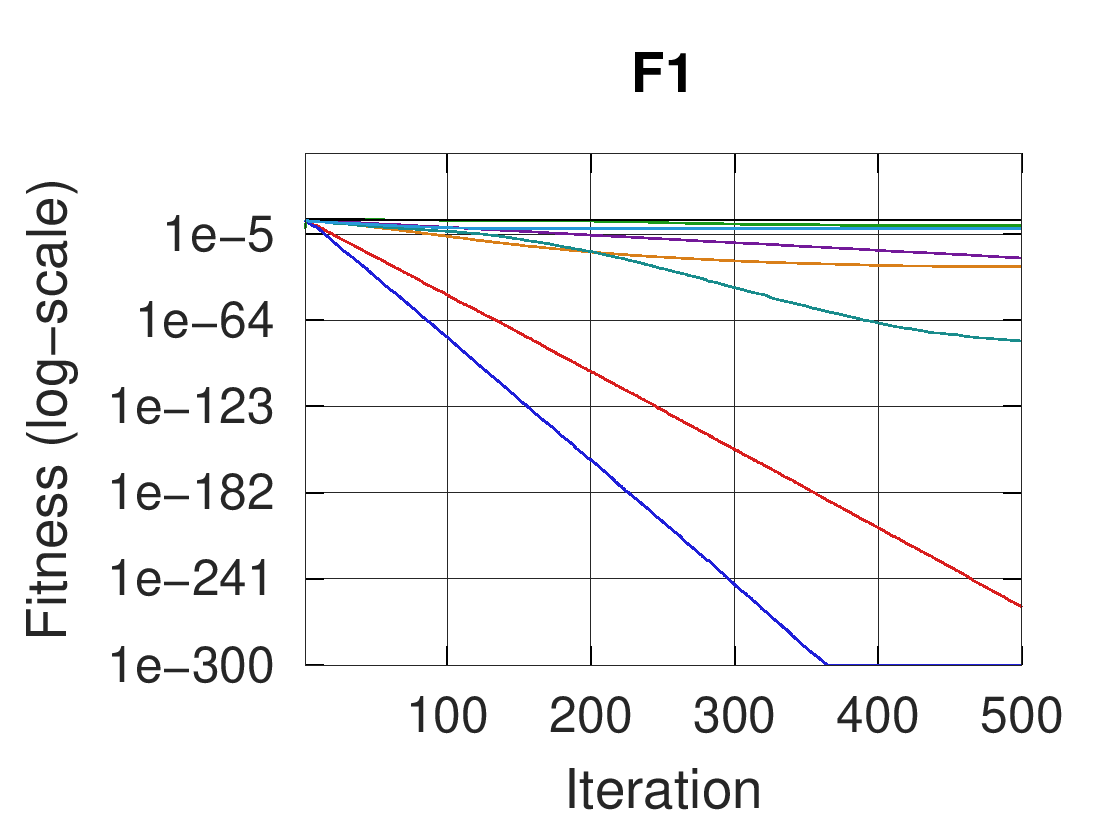
\includegraphics[width=\linewidth]{Pictures/convergence_F1.png}
    \caption{F1}
    \label{fig:conv-F1}
  \end{subfigure}\hfill
  \begin{subfigure}[t]{0.32\textwidth}
    \centering
    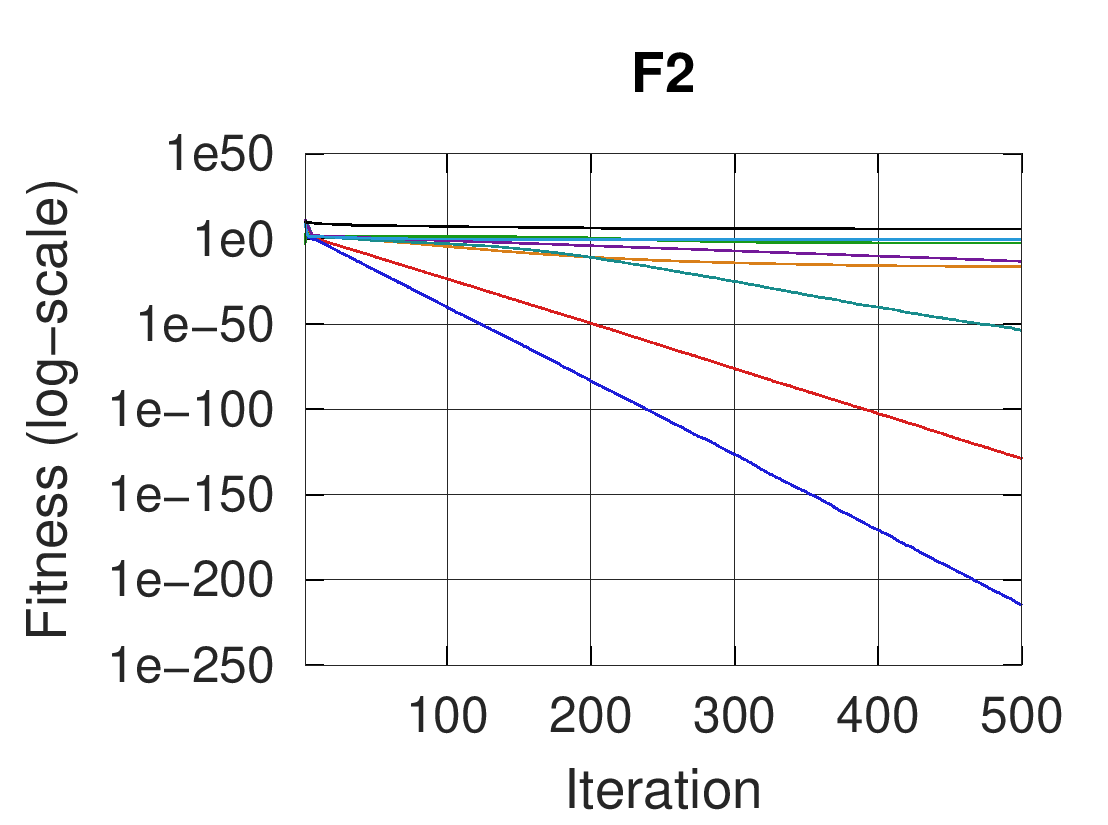
\includegraphics[width=\linewidth]{Pictures/convergence_F2.png}
    \caption{F2}
    \label{fig:conv-F2}
  \end{subfigure}\hfill
  \begin{subfigure}[t]{0.32\textwidth}
    \centering
    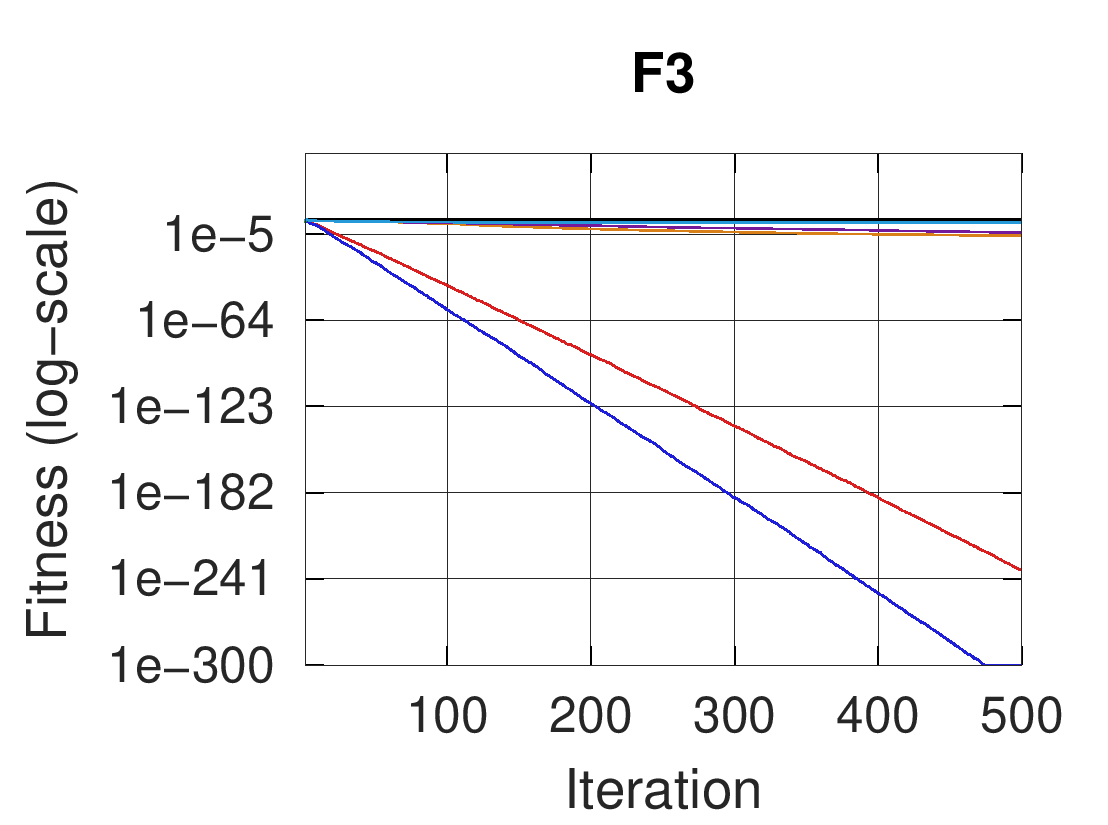
\includegraphics[width=\linewidth]{Pictures/convergence_F3.png}
    \caption{F3}
    \label{fig:conv-F3}
  \end{subfigure}

  \vspace{6pt}

  % ===== second row: F4 F5 F6 =====
  \begin{subfigure}[t]{0.32\textwidth}
    \centering
    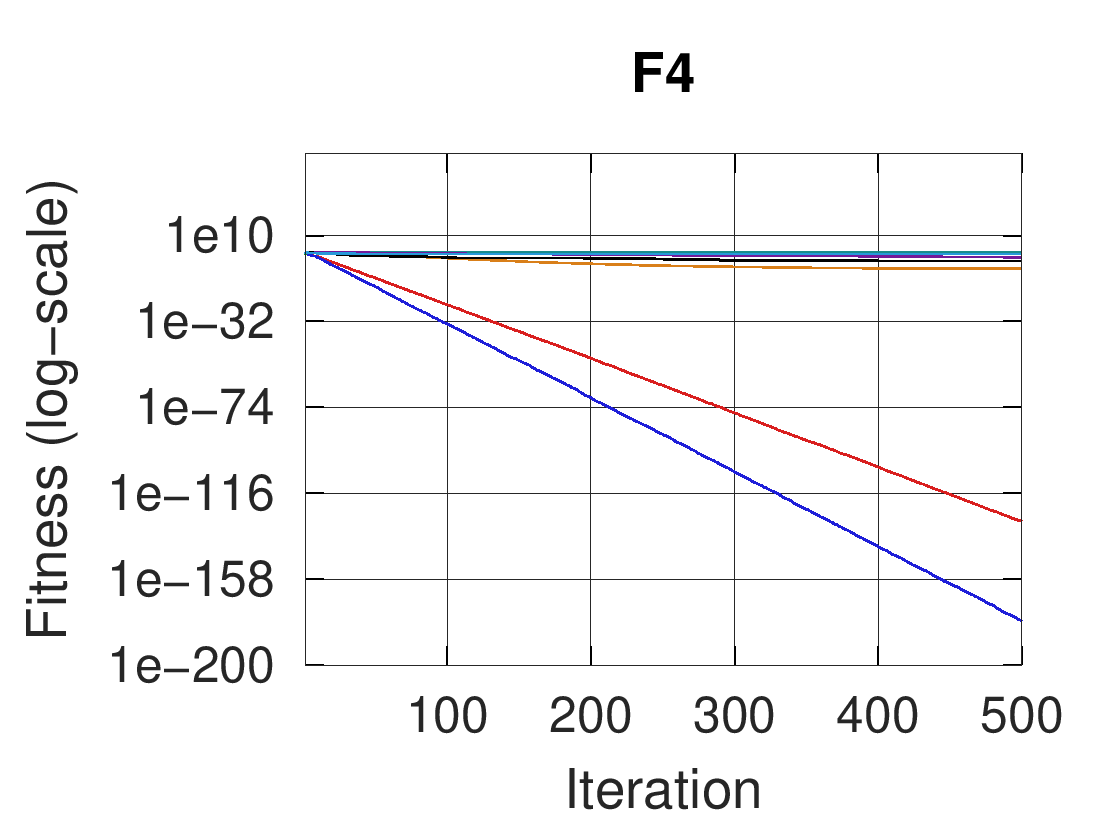
\includegraphics[width=\linewidth]{Pictures/convergence_F4.png}
    \caption{F4}
    \label{fig:conv-F4}
  \end{subfigure}\hfill
  \begin{subfigure}[t]{0.32\textwidth}
    \centering
    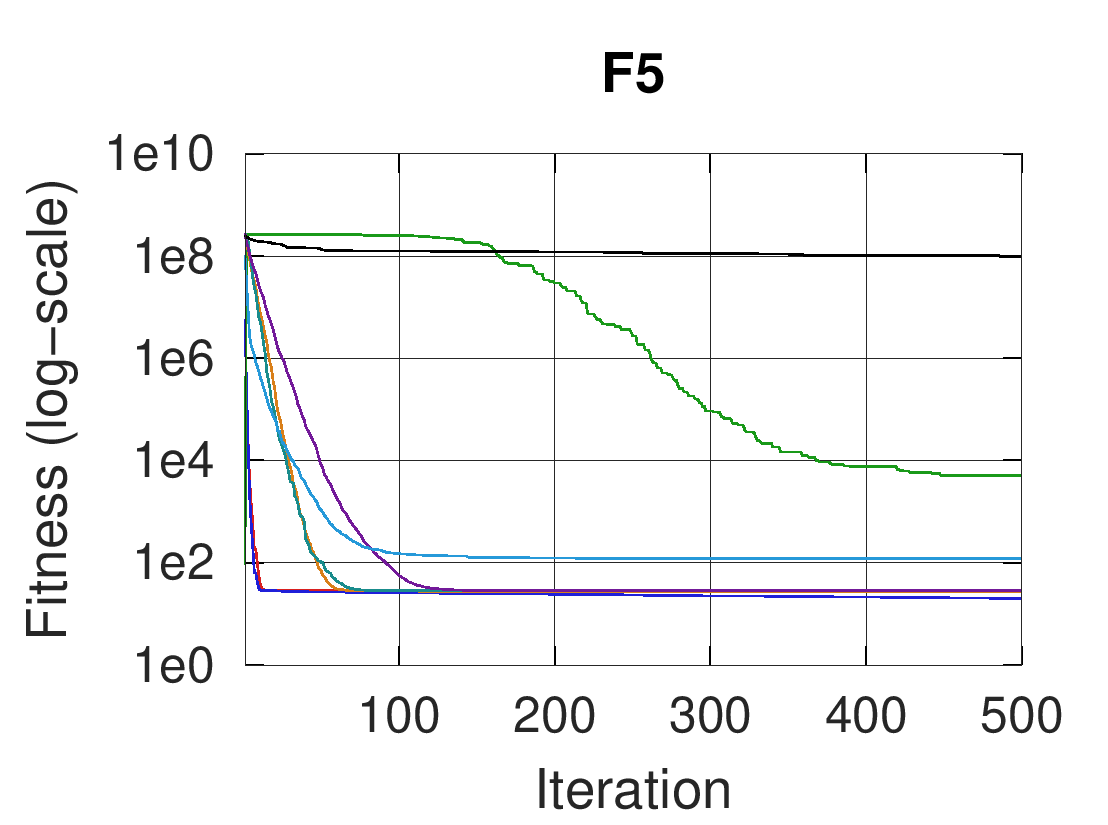
\includegraphics[width=\linewidth]{Pictures/convergence_F5.png}
    \caption{F5}
    \label{fig:conv-F5}
  \end{subfigure}\hfill
  \begin{subfigure}[t]{0.32\textwidth}
    \centering
    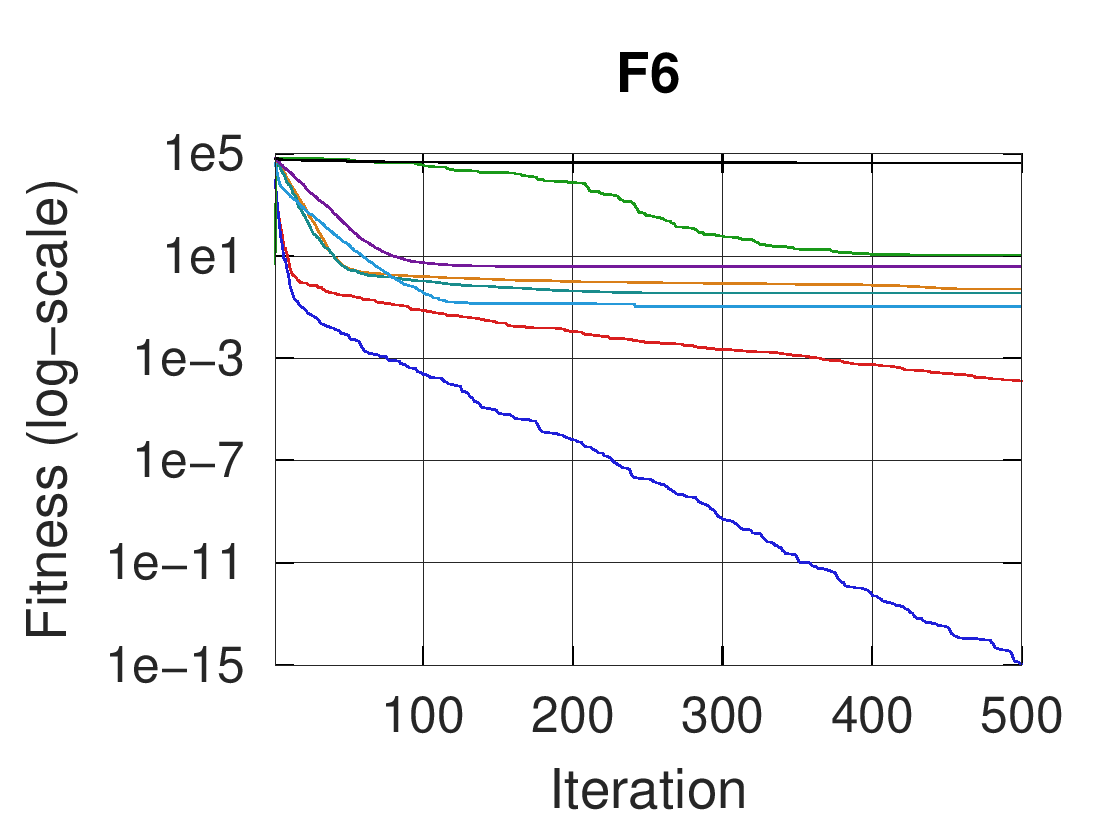
\includegraphics[width=\linewidth]{Pictures/convergence_F6.png}
    \caption{F6}
    \label{fig:conv-F6}
  \end{subfigure}

  \vspace{8pt}

  % ===== third row: centered F7 =====
  \begin{minipage}{0.32\textwidth}
    \centering
    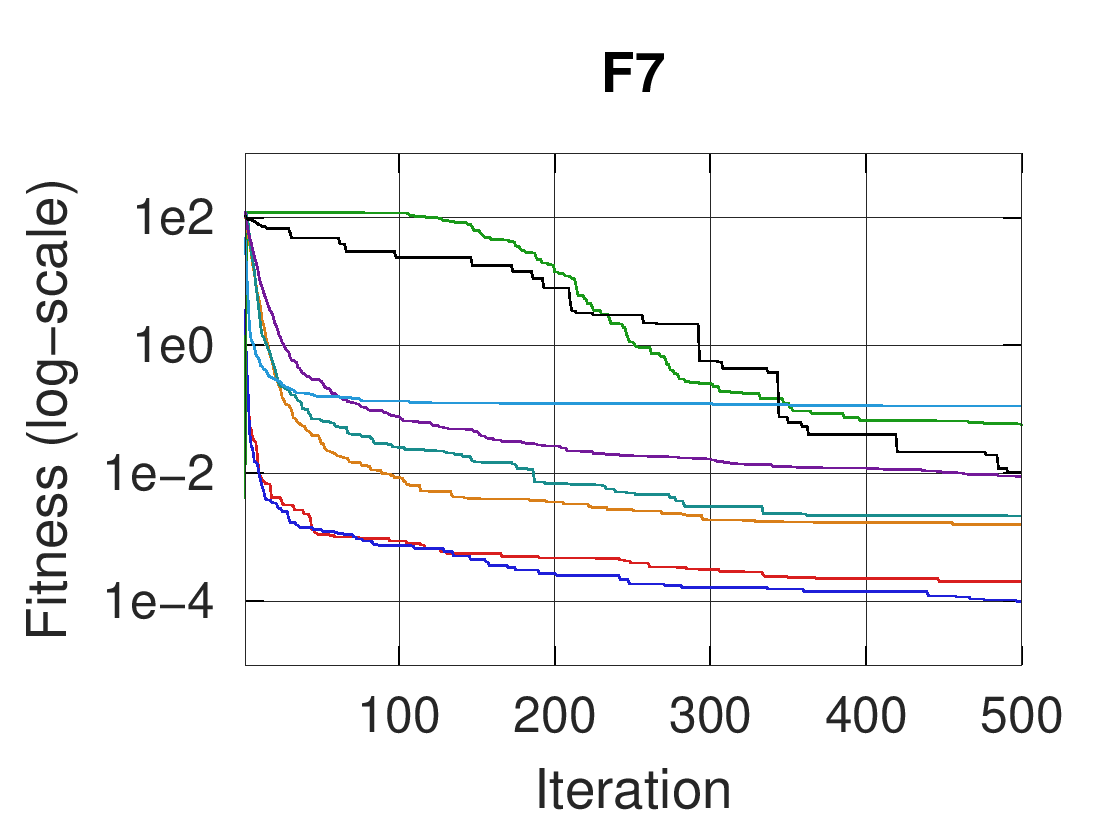
\includegraphics[width=\linewidth]{Pictures/convergence_F7.png}
    \caption*{\textbf{F7}}
    \label{fig:conv-F7}
  \end{minipage}

  \vspace{8pt}

  % ===== legend image centered beneath F7 =====
  \begin{minipage}{0.5\textwidth}
    \centering
    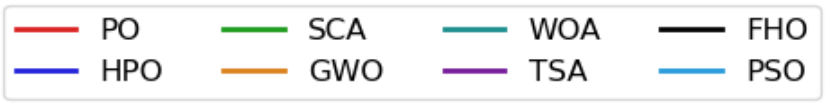
\includegraphics[width=0.95\linewidth]{Pictures/legend.png}
    % no caption for the legend image (or use caption* if you prefer)
  \end{minipage}

  \caption{Convergence curves (median best-so-far) for benchmark functions F1–F7. Each subplot shows the median convergence curve across independent runs for the algorithms compared. The legend (separate image) is shown below to keep the figure compact and publication-friendly.}
  \label{fig:convergence-grid}
\end{figure}
\FloatBarrier

\subsection{Summary of Findings}
\label{sec:summary-findings}

Across all unimodal and multimodal benchmark functions, the proposed Hybrid PUMA–PSO algorithm demonstrated superior optimization performance compared to the original PUMA and six state-of-the-art algorithms (SCA, GWO, WOA, TSA, FHO, and PSO). 
The hybridization of PUMA with PSO improved exploitation intensity without compromising exploration diversity, as evidenced by smoother convergence curves, lower mean fitness, and statistically significant gains in most functions. 
This confirms that incorporating a PSO-based refinement phase after PUMA’s exploitation stage effectively mitigates premature convergence and enhances local search accuracy. 
The consistency of improvements across varied landscapes suggests that Hybrid PUMA–PSO is both versatile and computationally efficient, making it well-suited for further deployment in VANET optimization tasks discussed in the next section.

\section{Applications of the Proposed Hybrid PUMA–PSO Optimizer}
\label{sec:applications}

Metaheuristic algorithms, owing to their flexibility and population-based search behavior, have demonstrated strong potential across numerous real-world optimization domains. 
While the original PUMA optimizer has been successfully applied to machine learning and classification tasks, the improved Hybrid PUMA–PSO variant is particularly suitable for dynamic and high-dimensional optimization problems that require a balance between global exploration and local refinement. 
This section outlines potential application areas, with special emphasis on route optimization in Vehicular Ad-hoc Networks (VANETs), where efficient path selection and adaptive decision-making are critical.

\subsection{Route Optimization in VANETs}
Vehicular Ad-hoc Networks (VANETs) are characterized by highly dynamic topologies, frequent node mobility, and rapidly changing communication links. 
One of the most challenging aspects of VANET design is the \textit{optimal route selection} problem, which directly impacts packet delivery ratio, end-to-end delay, and overall network throughput. 
Traditional deterministic routing protocols (such as AODV or DSR) often fail to adapt effectively to such dynamic environments. 
Hence, there is a growing interest in deploying nature-inspired metaheuristic algorithms for adaptive route optimization.

The proposed Hybrid PUMA–PSO algorithm can be effectively integrated into the routing decision process to optimize path selection based on multiple criteria—such as link stability, vehicular density, signal strength, and expected transmission delay. 
In this framework, each candidate route can be treated as a solution vector, and the optimization objective is to minimize a composite cost function that balances delay, hop count, and link reliability. 
PUMA’s exploratory behavior enables the discovery of globally promising paths across the vehicular topology, while PSO’s exploitation component refines these solutions locally to ensure stability and minimal route breaks.

By continuously updating the routing table using the best solutions obtained through Hybrid PUMA–PSO, the VANET can dynamically adapt to environmental changes such as vehicle speed, direction, and network congestion. 
This approach enhances both the robustness and scalability of VANET communications compared to conventional heuristics and standalone metaheuristics.

\subsection{Other Potential Applications}
Beyond VANETs, the proposed hybrid algorithm can be employed in several other complex optimization domains, including:
\begin{itemize}
    \item \textbf{Feature selection in machine learning:} selecting optimal feature subsets while reducing model complexity.
    \item \textbf{Image segmentation and computer vision:} optimizing segmentation thresholds and cluster centers.
    \item \textbf{Energy management in wireless sensor networks:} minimizing total energy consumption while maintaining network coverage.
    \item \textbf{Scheduling and resource allocation:} solving dynamic load-balancing problems in cloud and edge computing systems.
\end{itemize}

The hybrid design, with its balanced search capabilities and convergence reliability, makes it suitable for high-dimensional, nonlinear, and multi-objective problems where traditional optimization methods fail to perform efficiently.

\subsection{Summary}
The integration of Hybrid PUMA–PSO into VANET route optimization represents a promising future research direction. 
Its adaptability to network dynamics, combined with low computational cost, makes it a viable candidate for real-time vehicular decision systems. 
The next phase of this research will involve the implementation of the proposed approach within a realistic VANET simulation environment (SUMO–NS3) to quantitatively evaluate improvements in routing stability, latency, and delivery performance.

\section{Future Scope}
\label{sec:future-scope}

The present study enhanced the exploitation capability of the PUMA optimizer 
through hybridization with Particle Swarm Optimization (PSO) and verified its 
superior performance on standard benchmark functions. 
Although the proposed Hybrid PUMA–PSO model demonstrated high robustness and accuracy, 
several promising research directions remain open for future work.

\subsection{Integration with VANET Routing}
A primary direction for future research is the application of Hybrid PUMA–PSO 
to \textbf{route optimization in Vehicular Ad-hoc Networks (VANETs)}. 
The optimization objectives can be extended to multi-criteria parameters such as:
\begin{itemize}
    \item Link stability and vehicle connectivity,
    \item Vehicular speed and direction variability,
    \item Traffic density and network congestion,
    \item End-to-end delay and packet delivery ratio.
\end{itemize}
The hybrid model can dynamically select optimal routes by balancing these conflicting 
objectives in real time. Integration with network simulators such as 
\textbf{SUMO} (Simulation of Urban Mobility) and \textbf{NS-3} will allow 
comprehensive evaluation of metrics like throughput, latency, and route reliability.

\subsection{ Adaptive and Intelligent Parameter Control}
Another key enhancement involves incorporating adaptive control mechanisms 
that adjust algorithmic parameters during execution. 
This includes:
\begin{itemize}
    \item Adaptive coefficients that fine-tune exploration and exploitation,
    \item Reinforcement learning-based agents to guide parameter updates,
    \item Fuzzy or self-learning strategies for balancing population diversity.
\end{itemize}
Such methods will enable Hybrid PUMA–PSO to automatically respond to 
changes in problem complexity and convergence behavior.

\subsection{Multi-objective and Domain Extensions}
Future research can also extend the current single-objective framework into a 
\textbf{multi-objective} setting, where competing goals such as 
minimizing delay, maximizing throughput, and reducing energy consumption 
are optimized simultaneously.  
In addition, Hybrid PUMA–PSO can be applied to various other domains, including:
\begin{itemize}
    \item Energy-efficient routing in wireless sensor networks,
    \item Feature selection and hyperparameter optimization in machine learning,
    \item Task scheduling and load balancing in edge/cloud computing systems.
\end{itemize}

\subsection{Theoretical and Analytical Studies}
Finally, deeper theoretical analysis will be conducted to examine the 
convergence behavior and computational complexity of the hybrid optimizer. 
This includes deriving mathematical bounds on convergence rate and runtime 
performance.  
Such analysis will help formalize the algorithm’s stability and scalability 
across problem domains.

\vspace{4pt}
\noindent
\textbf{Overall,} future work will focus on deploying the Hybrid PUMA–PSO 
algorithm in dynamic, real-time environments—bridging the gap between 
simulation-based optimization and practical deployment in 
\textbf{intelligent transportation and communication systems}.

\section{Conclusion}
\label{sec:conclusion}

This study presented the development and analysis of a Hybrid PUMA–PSO 
metaheuristic optimizer designed to overcome the exploitation limitations of 
the original PUMA algorithm. 
The hybridization framework integrates the exploration strength of PUMA with 
the refinement capability of Particle Swarm Optimization, enabling the algorithm 
to maintain population diversity while achieving faster and more stable convergence.

Comprehensive experiments on benchmark functions (F1–F7) demonstrated that 
the proposed Hybrid PUMA–PSO consistently outperforms the original PUMA and several 
state-of-the-art algorithms, including SCA, GWO, WOA, TSA, FHO, and PSO. 
Statistical significance tests and convergence analyses confirmed the algorithm’s 
ability to balance global search and local exploitation more effectively, yielding 
lower mean fitness values and smoother convergence behavior. 

The results validate that incorporating PSO after PUMA’s exploitation phase 
significantly enhances its capacity for local search and fine-tuning near the global optimum. 
This improvement establishes the Hybrid PUMA–PSO as a robust and adaptive optimizer 
suitable for complex, dynamic, and nonlinear optimization tasks.

In future work, the algorithm will be extended and integrated into 
\textbf{Vehicular Ad-hoc Networks (VANETs)} for intelligent route optimization. 
By dynamically optimizing parameters such as link stability, traffic density, and delay, 
the hybrid model can contribute to more efficient and resilient vehicular communication systems. 
Beyond VANETs, the proposed method also shows promise in domains such as 
machine learning, resource scheduling, and energy-aware networking.

Overall, the Hybrid PUMA–PSO algorithm successfully bridges the gap between 
exploration-oriented and exploitation-oriented metaheuristics, offering a 
computationally efficient and general-purpose optimization tool for real-world applications.

\nocite{*}
\bibliographystyle{IEEEtran}  % or elsarticle-num / plainnat as required by publisher
\bibliography{references}


\end{document}
